\documentclass[]{article}
\usepackage{lmodern}
\usepackage{amssymb,amsmath}
\usepackage{ifxetex,ifluatex}
\usepackage{fixltx2e} % provides \textsubscript
\ifnum 0\ifxetex 1\fi\ifluatex 1\fi=0 % if pdftex
  \usepackage[T1]{fontenc}
  \usepackage[utf8]{inputenc}
\else % if luatex or xelatex
  \ifxetex
    \usepackage{mathspec}
  \else
    \usepackage{fontspec}
  \fi
  \defaultfontfeatures{Ligatures=TeX,Scale=MatchLowercase}
\fi
% use upquote if available, for straight quotes in verbatim environments
\IfFileExists{upquote.sty}{\usepackage{upquote}}{}
% use microtype if available
\IfFileExists{microtype.sty}{%
\usepackage[]{microtype}
\UseMicrotypeSet[protrusion]{basicmath} % disable protrusion for tt fonts
}{}
\PassOptionsToPackage{hyphens}{url} % url is loaded by hyperref
\usepackage[unicode=true]{hyperref}
\hypersetup{
            pdfborder={0 0 0},
            breaklinks=true}
\urlstyle{same}  % don't use monospace font for urls
\usepackage{longtable,booktabs}
% Fix footnotes in tables (requires footnote package)
\IfFileExists{footnote.sty}{\usepackage{footnote}\makesavenoteenv{long table}}{}
\usepackage{graphicx,grffile}
\makeatletter
\def\maxwidth{\ifdim\Gin@nat@width>\linewidth\linewidth\else\Gin@nat@width\fi}
\def\maxheight{\ifdim\Gin@nat@height>\textheight\textheight\else\Gin@nat@height\fi}
\makeatother
% Scale images if necessary, so that they will not overflow the page
% margins by default, and it is still possible to overwrite the defaults
% using explicit options in \includegraphics[width, height, ...]{}
\setkeys{Gin}{width=\maxwidth,height=\maxheight,keepaspectratio}
\IfFileExists{parskip.sty}{%
\usepackage{parskip}
}{% else
\setlength{\parindent}{0pt}
\setlength{\parskip}{6pt plus 2pt minus 1pt}
}
\setlength{\emergencystretch}{3em}  % prevent overfull lines
\providecommand{\tightlist}{%
  \setlength{\itemsep}{0pt}\setlength{\parskip}{0pt}}
\setcounter{secnumdepth}{0}
% Redefines (sub)paragraphs to behave more like sections
\ifx\paragraph\undefined\else
\let\oldparagraph\paragraph
\renewcommand{\paragraph}[1]{\oldparagraph{#1}\mbox{}}
\fi
\ifx\subparagraph\undefined\else
\let\oldsubparagraph\subparagraph
\renewcommand{\subparagraph}[1]{\oldsubparagraph{#1}\mbox{}}
\fi

% set default figure placement to htbp
\makeatletter
\def\fps@figure{htbp}
\makeatother


\date{}

\begin{document}

\section{Capítulo 1. El problema}\label{capuxedtulo-1.-el-problema}

\subsection{Planteamiento del
problema}\label{planteamiento-del-problema}

En Colombia, se puede apreciar la baja accesibilidad de banda ancha en
zonas rurales, ya que de acuerdo con ``Estado de la banda ancha en
América Latina y el Caribe'' dado por la Comisión Económica para América
Latina y el Caribe {[}@cepal2017{]}, menos del 10\% de esta población
tiene accesibilidad a servicio de banda ancha en el territorio nacional.
Además, se espera que para los próximos años la comisión de regulaciones
de las Comunicaciones aumente el ancho de banda para las zonas rurales,
para el año 2020: 1 Mbps a 10 Mbps de bajada y de 512 Kbps a 1Mbps
{[}@crt2016{]}, lo cual, si comparamos esto con los datos actuales que
se tienen del ancho de banda en la red libre de Bosachoque
{[}@florez2018{]}, se puede evidenciar que no se alcanzara el nivel de
banda ancha, por lo tanto, es necesario modificar la red, y para esto
los Proveedores Inalámbricos de Servicios de Internet WISP solo pueden
tomar dos acciones para extender su cobertura de banda ancha, estas son
Incrementar la cobertura de red, o mejora las áreas ya existentes. En
ambos casos, estas acciones son limitadas por el presupuesto y solo un
pequeño conjunto de acciones pueden ser ejecutadas.

La planeación de redes se convierte en un proceso fundamental para estos
casos, sin embargo, existen gran cantidad de software para el
planeamiento de redes inalámbricas, pero estas herramientas a menudo no
están disponibles, ni tampoco son adecuados para comunicar pequeñas
comunidades y pequeños WISP (en este caso la Universidad de
Cundinamarca) {[}@bernardi2012{]}. El difícil acceso a herramientas de
planeación de redes inalámbricas limita la presencia de ISP en zonas
rurales ya que ellos no saben con certeza como invertir en
infraestructura que permita acceso a internet de banda ancha. Las
comunidades excluidas de la banda ancha corren el riesgo de quedar al
margen de toda una gama de aplicaciones y ventajas que proporciona
Internet, dejando a un lado la posibilidad de generar un desarrollo
económico {[}@onu2013{]}.

¿Cómo planificar la expansión estratégica de la Red Libre de Bosachoque
con un algoritmo de planificación de redes inalámbricas en zonas
rurales?

\subsection{Objetivos del estudio}\label{objetivos-del-estudio}

\subsubsection{Objetivo general}\label{objetivo-general}

Diseñar un algoritmo para la planeación incremental de redes
inalámbricas en áreas rurales evaluándolo en la red Libre de Bosachoque

\subsubsection{Objetivos específicos}\label{objetivos-especuxedficos}

\begin{itemize}
\item
  Generar el estado del arte de los algoritmos utilizados en la
  planeación de redes inalámbricas que permitan identificar y determinar
  los requerimientos del algoritmo que sugieran la mejor estrategia de
  expansión de una red
\item
  Diseñar un algoritmo que permita identificar la mejor estrategia de
  expansión de la red inalámbrica en zonas rurales
\item
  Evaluar el algoritmo mediante una simulación numérica, comparándolo
  con Heurística simple.
\item
  Aplicar el algoritmo diseñado en la red libre de Bosachoque analizando
  los resultados obtenidos
\end{itemize}

\subsection{Justificación}\label{justificaciuxf3n}

El acceso a Internet de banda ancha tiene impactos positivos en la
sociedad, puesto que contribuye de manera significativa al crecimiento
económico en muchos aspectos, ya que mejora la productividad, facilita
la adopción de procesos de negocio eficientes ,aumenta la innovación y
mejora los procesos de funcionamiento en las empresas {[}@uit2012{]},
por esta razón la Comisión de Ciencia y Tecnología para el Desarrollo de
las Naciones Unidas mediante su informe ``El acceso de banda ancha a
Internet como medio de lograr una sociedad digital inclusiva'' véase en
{[}@PNUD2018{]}, sugiere a todas las naciones miembros de la ONU
(``Organización de las Naciones Unidas'') aumentar los esfuerzos de que
todas las personas y comunidades tengan acceso a banda ancha. Sin
embargo, la falta de accesibilidad a banda ancha en zonas rurales se
debe a que los Proveedores de Servicios de Internet ISP, tienen que
desplegar su infraestructura en lugares donde probablemente no
retornaran su inversión, por esto, es importante planificar un óptimo
despliegue o actualización de la red. En la actualidad, se encuentran
toneladas de software para la planeación de redes, sin embargo, estas
están enfocadas al planeamiento de redes de banda ancha de telefonía
móvil {[}@hilarie2008{]} y redes inalámbricas locales WLAN (Bosio,
2008), mientras que para la planificación de redes BWA en zonas rulares
estos enfoques son limitados por la comunidad de investigación.

Nuestro enfoque está basado en las necesidades de guiar WISP en áreas
rurales que se enfrentan con el único reto de extender su rendimiento
con inversiones estrechas en un ambiente de ganancias limitadas. La
clave para tales organizaciones es identificar la estrategia de
despliegue más económica para planear su red mientras se toma en
consideración su cobertura. Por esto, en el presente anteproyecto, se
propone el diseño de un algoritmo de optimización, que permita
identificar el camino de solución de menor costo, seguido del desarrollo
de un software que permita mostrar visualmente las posibles acciones a
seguir, para finalmente, implementar el presente software en la Red
Libre de Bosachoque, en donde se evaluará los resultados.

\subsubsection{Beneficios
tecnológicos}\label{beneficios-tecnoluxf3gicos}

Se dará a conocer una nueva perspectiva a las WISP en la planificación
de redes BWA en zonas rurales, incentivando la conectividad y
accesibilidad a la banda ancha, además de que tendrá accesibilidad a la
herramienta , puesto que se tiene previsto el desarrollo de un software
libre, el cual podrá ser propenso a actualizaciones o mejoras por parte
de la comunidad tecnológica, además de que fomentará la posibilidad de
generar otras herramientas de software para la solución de problemas de
optimización y planeación de redes.

\subsubsection{Beneficios
institucionales}\label{beneficios-institucionales}

El desarrollo del proyecto permitirá al programa de ingeniería
electrónica de la Universidad de Cundinamarca a contar con una
herramienta que permita el desarrollo económico de la comunidad rural
del municipio (vereda de Bosachoque) y demás lugares donde esta
herramienta se pueda implementar, además que permitirá mejorar el
servicio como WISP, que presta la Universidad en la Red Libre de
Bosachoque. También permitirá el fortalecimiento del semillero de
investigación Kinestasis, fomentando el desarrollo de herramientas
tecnológicas al servicio de la sociedad.

\subsubsection{Beneficio social}\label{beneficio-social}

La herramienta permitirá sugerir las mejores decisiones al momento de
planear una red o mejorar la cobertura de Internet de banda ancha,
llevando consigo un desarrollo económico, puesto que la comunidad podrá
tener a su disponibilidad un sin fin de herramientas que permitan
generar un desarrollo económico en el entorno, además de fortalecer el
sector rural y disminuir la brecha digital que existe en los países en
desarrollo.

\subsection{Alcances y limitaciones}\label{alcances-y-limitaciones}

\subsubsection{Alcances}\label{alcances}

El presente proyecto tiene como objeto diseñar un algoritmo para la
planeación incremental de redes inalámbricas que permita sugerir las
mejores opciones para incrementar la cobertura de ancho de banda y
acceso a internet en zonas rurales. Este algoritmo se implementará y
evaluará en la red libre comunitaria de Bosachoque, se espera que sea
una herramienta adecuada que permita la toma de decisiones al momento de
planificar la expansión de la red, además se plantea la base para
desarrollar futuros trabajos en el campo de las redes y las
telecomunicaciones como puede ser el diseño de un software.

\subsubsection{Limitaciones}\label{limitaciones}

El proyecto estará limitado por la infinidad de soluciones válidas para
realizar la planeación incremental de una red ya que se pueden generar
problemas de algoritmos como bucles infinitos, NP-hard, entre otros. En
la evaluación se tiene limitaciones en cuanto a infraestructura
disponible para desplegar torres nuevas, nodos nuevos, ampliación de
nodos, y demás acciones sugeridas por la herramienta.

\section{Capítulo 2. Marco
referencial}\label{capuxedtulo-2.-marco-referencial}

\subsection{Antecedentes}\label{antecedentes}

El acceso a Internet a través de las tecnologías de la información y las
comunicaciones (TIC) se ha convertido en un instrumento fundamental de
desarrollo social, económico, político y cultural para los gobiernos y
sociedades en todo el mundo, lo que ha conllevado a un desarrollo
digital.

El desarrollo digital hace referencia a aspectos como Infraestructuras
que faciliten el acceso universal, geográfico y social a las
tecnologías; sector TIC respecto a la industria tecnológica existente;
competencias digitales o nivel de alfabetización digital en un tiempo
determinado; marco legal y regulatorio referente a normatividad,
políticas y estrategias de las TIC; contenidos y servicios que incluye
la oferta de servicios digitales{[}@maseratti2011{]}.

Aunque la era digital es un fenómeno mundial existente en países más
desarrollados que otros, conlleva a la denominada brecha digital que es
la ausencia de una o varias dimensiones contenidas en el desarrollo
digital, es esta entonces un reto para la sociedad de la información.

Una alternativa para disminuir la brecha digital, son las redes Libres
comunitarias (RLC), entendidas no solo como redes de computadores sino
como redes comunitarias implementadas en poblaciones vulnerables donde
el acceso a la información es una posibilidad y no una realidad
{[}@gordillo2013{]}.

Debido a que las redes comunitarias por lo general se encuentran
desplegadas en áreas geográficamente separadas, se utilizan tecnologías
inalámbricas como mesh y radioenlaces usando bandas libres como la de
2,4 GHz; Las tecnologías inalámbricas son ampliamente utilizadas en
áreas rurales, ya que, por cuestiones de acceso e infraestructura, las
tecnologías cableadas no resultan ser viables para estos casos, dando
como solución las redes inalámbricas comunitarias (WCN)
{[}@flickenger2008{]} . Además, en este tipo de redes, se emplean
materiales que pueden ser adquiridos por la comunidad, y donde este
autor muestra una guía detallada para realizar conexiones inalámbricas,
que permitan conectar con un ancho de banda significativo lugares
remotos y de difícil acceso, además de tener un enfoque orientado a
países en desarrollo. En varias partes del mundo se pueden encontrar
diferentes redes comunitarias, un ejemplo bastante significativo y de
gran éxito es la red guifi.net, que comenzó en 2004 en la comarca de
Osona (Catalunya), este es un proyecto tecnológico, social y económico,
impulsado desde la ciudadanía que tiene por objetivo la creación de una
red de telecomunicaciones abierta, libre y neutral, basada en un modelo
de procomún {[}@guifi.net2016{]}. Guifi.net tiene a la fecha de
diciembre de 2016, 32.500 nodos activos y se calcula que más de 50.000
personas reciben servicio de Internet gracias a esta red. Sin embargo,
el éxito de esta red no radica especialmente en la gran cobertura que
ofrece y de cómo ha sido el impacto en los países en que se ha
desarrollado, sino que según (Roger,2015), ha permitido mostrar la
importancia de mantener la infraestructura de la red como bien colectivo
ya que el principio subyacente detrás de guifi.net es la firme
convicción de que la mejor manera de mantener una red es estableciéndola
como un recurso colectivo común (CPR).

A pesar que gran parte de los nodo están conectados con tecnología WiFi
en Guifi.net, también utiliza tecnología cableada y de fibra óptica,
debido a que se desarrolló en gran parte en zonas urbanas, sin embargo
como ya hemos mencionado, la WCN ha tenido gran participación en zonas
rurales, en este enfoque se destaca una red inalámbrica mesh (WMN),
desplegada por la universidad de Lancaster en Wray (Inglaterra),
proporcionando servicio de Internet a una villa en un área aproximada de
dos kilómetros por un periodo de tres años {[}@ishmael2008{]}. Esto a
pesar de haber tenido algunas limitaciones y complicaciones, muestra
cómo se tuvo que reeducar a la gente para que se pueda hacer uso de la
red de la mejor manera, dando como resultado la disponibilidad de banda
ancha y mejorando la calidad de los servicios que se prestan.

En el ámbito local, en Bogotá se han desplegado diferentes redes
inalámbricas comunitarias, las cuales valen la pena resaltar a pesar de
no ser un entorno rural, estas muestran la forma de cómo se puede hacer
inclusión social a sectores populares, en esta aparece
{[}@pedraza2012{]}, una red desplegada desde la Universidad Francisco
José de Caldas, la cual muestra desde el proceso de selección de puntos
donde se desplegaron los nodos, hasta la evaluación de los resultados
después de su despliegue; en esta investigación se logró ampliar la
cobertura en más de 40\% con el uso de antenas artesanales, utilizando
guías y herramientas propuestas por {[}@flickenger2008{]} , demostrando,
que la participación de la ciudadanía es fundamental para el éxito de
estas redes.

\subsubsection{Descripción de la red de Bosachoque
Libre}\label{descripciuxf3n-de-la-red-de-bosachoque-libre}

La Red Bosachoque Libre es un macroproyecto misional de investigación de
la Universidad de Cundinamarca de Facultad de Ingeniería (redes libres
como alternativa de innovación social e inclusión digital en la vereda
Bosachoque del municipio de Fusagasugá), con el fin de proveer servicio
de Internet a la vereda Bosachoque utilizando conexiones inalámbricas,
dado que, por ser una zona rural, una conexión cableada sería costosa y
difícil. Esta red, se implementó con el fin de generar a la comunidad
una herramienta que permita la conectividad, fomentando el desarrollo y
crecimiento de esta, utilizando las tecnologías, protocolos y
herramientas típicas de una red inalámbrica en países en desarrollo. El
proceso de cómo se planeó esta red se encuentra documentado en
{[}@achury2018{]}.

La red de Bosachoque fue planeada e implementada como una red BWA
(acceso inalámbrico de banda ancha ``Broad Band Wireless Access'') de
dos niveles, nivel de back-haul donde de manera inalámbrica se adquiere
el servicio de internet y nivel de acceso donde se conectan los usuarios
finales. El nivel back-haul hace referencia a los sitios de transmisión
que están interconectados usando enlaces inalámbricos punto a punto de
larga distancia (PTP), mientras que el nivel de acceso proporciona
conectividad al equipo del cliente (CPE) a través de un enlace punto
multipunto (PMP).

La universidad de Cundinamarca sede Fusagasugá hace la función de
proveedor de servicio de Internet (ISP) con el fin de desarrollar y
ejecutar el macroproyecto mencionado.

Para el diseño, se especificó un DNS, este se tomó a partir del DNS
asignado a la universidad de Cundinamarca, el cual es 200.14.41.2 y,
como respaldo se utilizó el DNS de Google 8.8.8.8, además, la red cuenta
con servicios de DHCP y firewall, cumpliendo con las especificaciones de
enrutamiento y seguridad que una red de esta magnitud debe tener.

El dimensionamiento del número de usuarios se estableció según el POT
(plan deordenamiento territorial) 2014, cuyos datos reposan de manera
oficial en la alcaldía de Fusagasugá, donde se consta que en esta
población rural se encuentran un número aproximado de 4000 personas, por
ende, el direccionamiento está diseñado para suplir de servicio de
Internet a la comunidad a un total de 4000 Host.

En este nivel se utiliza un enrutador y una antena Access Point ubicada
en la Universidad de Cundinamarca específicamente en el bloque F, donde
por medio de un enlace punto a punto (PTP) y utilizando dos antenas
RocketM5 AC a una frecuencia de trabajo entre 5.2 GHz 5.8 GHz , se
direcciona a un punto ubicado en la vereda san José del chocho del
municipio de Silvania-Cundinamarca; Aquí se encuentra el nivel de acceso
, donde un enlace multipunto con topología anillo se encarga de la
distribución de la señal por medio de una antena sectorial Rocket Prism
AC, a todas las subredes que se encuentra dentro de la vereda Bosachoque
(Tobón).

\subsection{Marco Teórico}\label{marco-teuxf3rico}

\subsubsection{Brecha Digital}\label{brecha-digital}

En el año 1995 eclosionan para la población dos tecnologías totalmente
disruptivas, Internet y la telefonía móvil, ellas sugieren una nueva
revolución, la llamada revolución digital, que a su vez crea la sociedad
de la información (S.I), dando inicio al planteamiento sobre cómo medir
y modelizar la S.I, el nivel de desarrollo digital y el impacto del
desarrollo digital en el ser humano. De igual manera, el acceso a
Internet a través de las Tecnologías de la Información y las
Comunicaciones (TIC) ha tenido un auge exponencial en los últimos años,
en efecto, este avance se presenta en países desarrollados o zonas
metropolitanas de países en desarrollo (@sen2007), sin embargo, existen
unas comunidades con poco o ningún acceso a las TIC {[}@maseratti2011{]}
y otras con acceso casi universal a telefonía fija, móvil e Internet de
banda ancha, es así que resulta el concepto de \textbf{brecha digital}
entendiéndose como la ausencia de una o varias dimensiones contenidas en
el desarrollo digital. En relación con lo anterior, las poblaciones sin
acceso a las TIC poseen un bajo nivel socioeconómico, viven en zonas de
difícil acceso con condiciones climatológicas desfavorables e incluso
con ineficiencia o inexistencia de redes eléctricas, al mismo tiempo,
las personas que viven en áreas rurales sufren el efecto de la brecha
digital incluso más fuerte que los habitantes urbanos, debido a que no
pueden acceder a servicios como el aprendizaje a distancia, la salud y
el comercio electrónico (@bernardi2012).

\begin{figure}
\centering
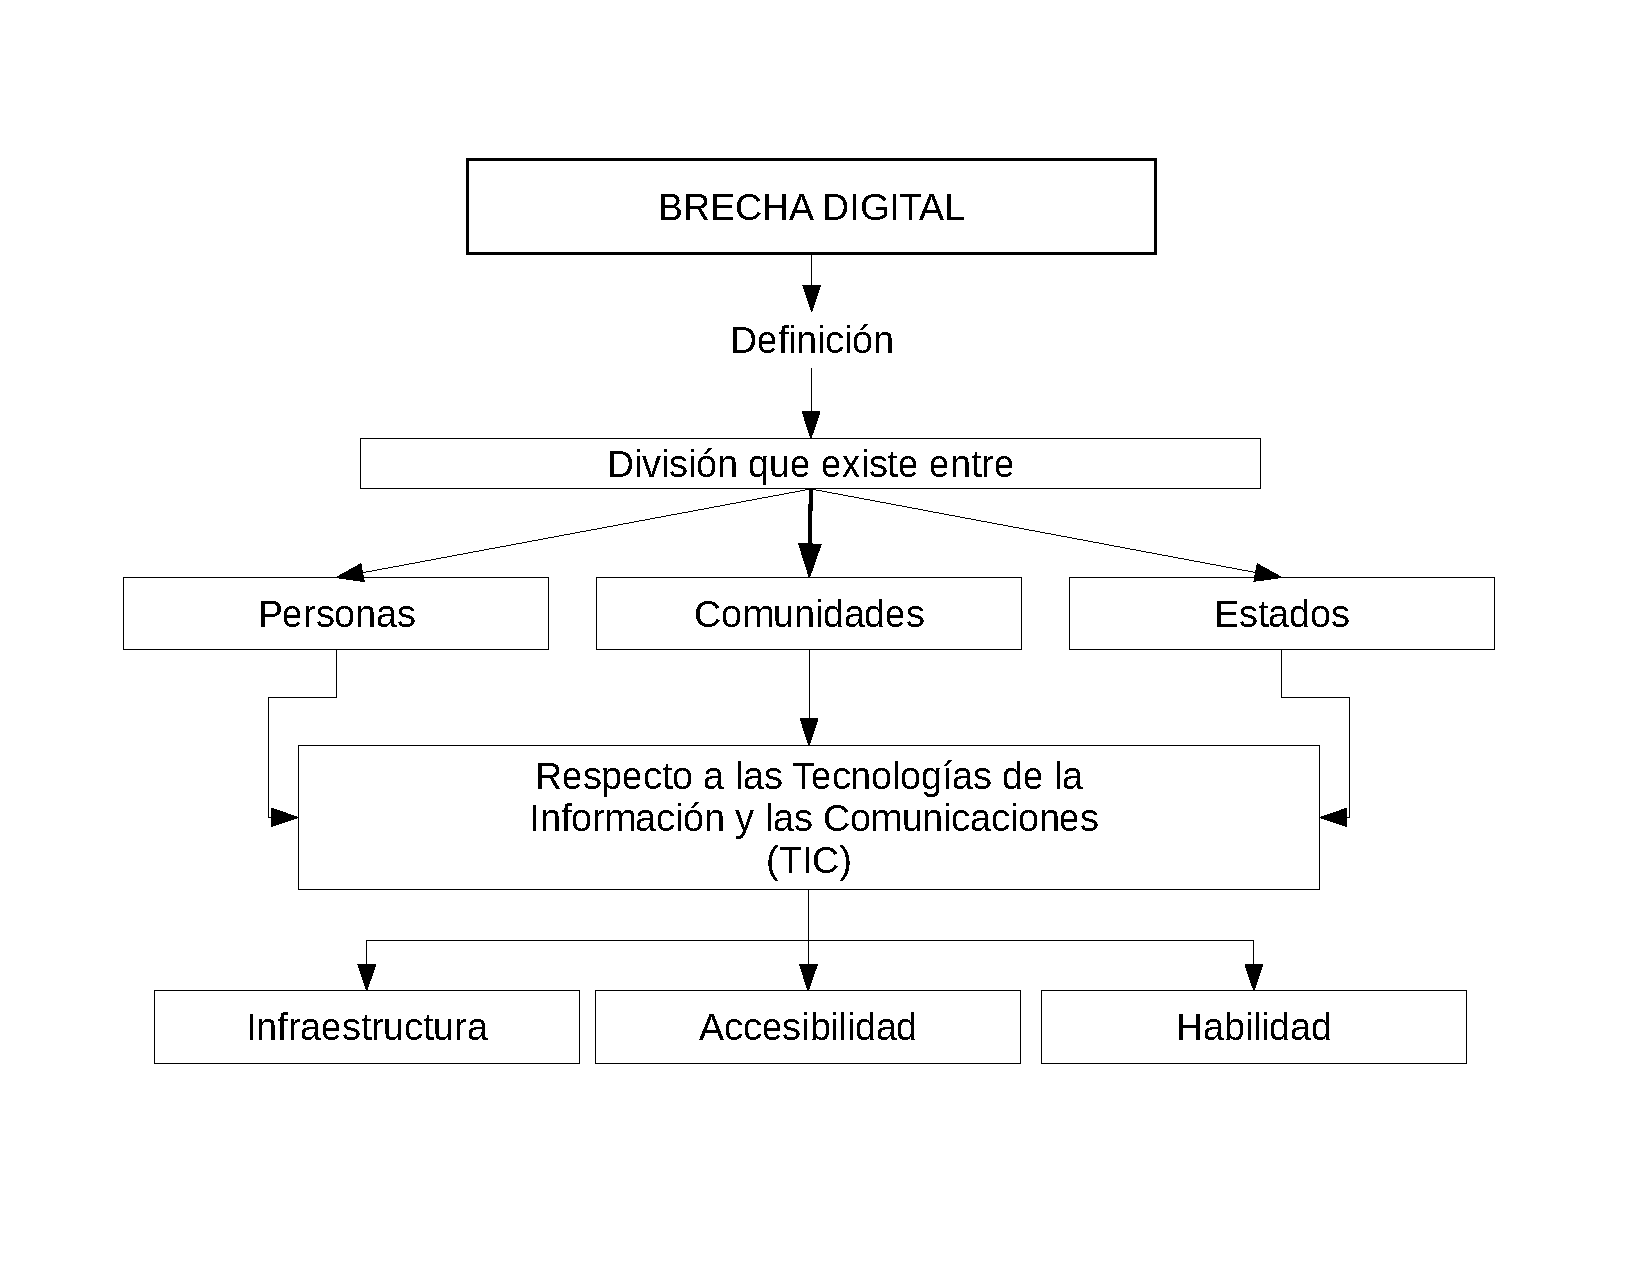
\includegraphics{imagen_brdigital.pdf}
\caption{Brecha Digital}
\end{figure}

La ilustración 1 enmarca la definición de Brecha Digital en donde se
aprecia que es la separación entre personas, comunidades y estados que
tienen o no acceso a las Tecnologías de las Información y las
Comunicaciones debido a la falta de infraestructura, difícil acceso a
zonas apartadas de centros poblados y su nivel de alfabetización
digital.

\subsubsection{Redes Libres
Comunitarias}\label{redes-libres-comunitarias}

Una alternativa para disminuir la brecha digital, son las Redes Libres
Comunitarias (RLC), entendidas no solo como redes de computadores sino
como redes comunitarias implementadas en poblaciones vulnerables donde
el acceso a la información es una posibilidad y no una realidad
(@gordillo2013).

Una red libre comunitaria, es una red troncal, dividida en subconjuntos
de redes construidas y gestionadas de manera colectiva por la comunidad,
la cual se involucra en la red de forma activa y participativa.

\paragraph{Principios generales}\label{principios-generales}

\begin{itemize}
\item
  Libertad de utilizar la red para cualquier propósito mientras no se
  perjudique el funcionamiento de la propia red, la libertad de otros
  usuarios, y se respete las condiciones de los contenidos y servicios
  que circulan libremente.~
\item
  Libertad de conocer como es la red, sus componentes y su
  funcionamiento, también se puede difundir su espíritu y funcionamiento
  libremente.
\item
  Libertad para incorporar servicios y contenidos a la red con las
  condiciones que se quiera.
\item
  Libertad de Incorporarse a la red y ayudar a extender estas libertades
  y condiciones. (@guifi.net2016)~
\end{itemize}

\paragraph{Características de RLC}\label{caracteruxedsticas-de-rlc}

\begin{itemize}
\item
  Abiertas: porque todo el mundo tiene el derecho a conocer la forma en
  que se construyen.
\item
  Libres: ya que el acceso a esta red está impulsado por un principio de
  no discriminación, por lo que son de acceso universal.
\item
  Neutrales: porque cualquier solución técnica disponible se puede
  emplear para ampliar la red, y porque la red se puede utilizar para
  trasmitir datos de cualquier tipo por cualquier participante,
  incluyendo también fines comerciales(@guifi.net2016).
\end{itemize}

Debido a que las redes comunitarias por lo general se encuentran
desplegadas en áreas geográficamente separadas, se utilizan tecnologías
inalámbricas como mesh y radioenlaces usando bandas libres como la de
2,4 GHz; las tecnologías inalámbricas son ampliamente utilizadas en
áreas rurales, ya que, por cuestiones de acceso e infraestructura, las
tecnologías cableadas no resultan ser viables para estos casos, dando
como solución las redes inalámbricas comunitarias (WCN) en donde ya se
han realizado trabajos importantes como se muestra en (@flickenger2008).

\subsubsection{Planeación de Redes
Inalámbricas}\label{planeaciuxf3n-de-redes-inaluxe1mbricas}

Una red inalámbrica es la interconexión de varios nodos entre sí
mediante la transmisión y recepción de señales electromagnéticas sin
ninguna guía, empleando como medio el aire o el espacio vacío. La
planificación de redes supone la definición de requisitos para la
creación de una infraestructura que permita conectar estos sistemas a
través de una red (@IBM2019), se debe agregar que, la planeación de
redes inalámbricas es un área muy activa por la comunidad científica,
sin embargo, el foco de las investigaciones son las redes de banda ancha
móvil y redes de área local inalámbrica.

\paragraph{Factores clave de la
planeación}\label{factores-clave-de-la-planeaciuxf3n}

A continuación, se detallan factores claves de la planeación de redes
inalámbricas.

\begin{itemize}
\item
  Costos de despliegue: valor inicial de instalación de la red.
\item
  Costos de implementación: coste del mantenimiento y funcionamiento de
  la red.
\item
  Expansión de la red: crecimiento de la red, abarcando más territorio.
\item
  Cobertura de la red: área geográfica que cubre la red.
\item
  Capacidad de la red: ancho de banda requerido para la transferencia de
  datos.
\item
  Retorno de la inversión: beneficio obtenido en relación a la inversión
  realizada.
\end{itemize}

\subsubsection{Algoritmos utilizados en la
planeación}\label{algoritmos-utilizados-en-la-planeaciuxf3n}

Aunque existen estructuras de algoritmos para solucionar problemáticas
en la planeación incremental de redes inalámbricas {[}@Whitaker{]}
proporcionan información acerca de los enfoques propuestos para el
diseño de redes, que muestran la evolución de modelos y técnicas para la
planificación automática de servicios inalámbricos celulares, cabe
resaltar que la documentación existente hace énfasis en redes móviles,
sin embargo, este concepto es aplicable para el despliegue de redes
inalámbricas rurales. Dicho lo anterior, \emph{Whitaker} facilita la
descripción de diferentes clases de algoritmos que se pueden usar para
realizar la planeación de redes inalámbricas.

\begin{itemize}
\tightlist
\item
  \textbf{Algoritmos voraces}
\end{itemize}

Es una estrategia de búsqueda por la cual se sigue una heurística
consistente en elegir la opción óptima en cada paso local con la
esperanza de llegar a una solución general óptima. El procedimiento
central del algoritmo voraz apunta a asignar las mejores ubicaciones
posibles a un conjunto dado de estaciones base activas.

\begin{itemize}
\tightlist
\item
  \textbf{Algoritmos genéticos (GA)}
\end{itemize}

Estos algoritmos imitan algunos de los procesos de evolución y selección
natural al mantener una población de soluciones candidatas que están
representadas por una cadena de genes (con frecuencia binarios). Con el
tiempo, la población evoluciona a través de procesos que emulan procesos
biológicos como la reproducción. Los miembros de la población se
combinan para producir descendientes. El concepto básico es que los
fuertes tienden a adaptarse y sobrevivir, mientras que los débiles
tienden a desaparecer. En la planeación de redes se utiliza la
optimización de varios objetivos, estos se conocen como optimización
multiobjetivo, en la que existe más de una solución óptima con respecto
a todos los objetivos, entre ellos lugar de instalación de una torre,
configuración de una antena,asignación de altura, etc.

\begin{itemize}
\tightlist
\item
  \textbf{Búsqueda tabú (TS)}
\end{itemize}

La búsqueda tabú es un algoritmo heurístico de nivel superior para
resolver problemas de optimización combinatoria. Es un procedimiento de
mejora iterativo que comienza a partir de cualquier solución inicial y
trata de determinar una mejor solución. TS (por sus siglas en inglés
\emph{tabu search}) se caracteriza por su capacidad para evitar el
atrapamiento en la solución óptima local y para evitar los ciclos,
utiliza una memoria visible del historial de búsqueda. Normalmente, el
algoritmo TS comienza sin conocer la solución correcta, dependiendo
completamente de las respuestas del entorno que interactúa para llegar a
la solución óptima (@Abido2002). Este algoritmo permite encontrar una
ubicación de las torres en la fase de planeación para lograr un óptimo
rendimiento de la red.

\subsubsection{Representación de la
topología}\label{representaciuxf3n-de-la-topologuxeda}

Topología se refiere a la configuración de la red, es decir, a su forma
de conectividad física en la que los dispositivos intercambian datos
entre sí.

Para diseñar la infraestructura de la topología de la red requerida, es
necesario describir la topología por medio del uso de grafos ya que es a
través de esta estructura de datos que se elabora el procesamiento
computacional del problema (@rios2015)

\paragraph{Grafo}\label{grafo}

Un grafo en el ámbito de las ciencias de la computación es un tipo
abstracto de datos (TAD), que consiste en un conjunto de nodos (también
llamados vértices) y un conjunto de arcos (aristas) que establecen
relaciones entre los nodos. Formalmente se representa mediante el par
\(G=(V, A)\), dónde:

\begin{itemize}
\item
  \(V\) es un conjunto de objetos llamados vértices o nodos.
\item
  \(A\) es un conjunto de objetos denominados aristas o arcos.
\item
  Las aristas representan relaciones entre los vértices, de forma que
  una arista es un par \((u,v)\) de vértices de \(V\).
\end{itemize}

\subparagraph{Herramientas de manipulación de
grafos}\label{herramientas-de-manipulaciuxf3n-de-grafos}

\begin{itemize}
\tightlist
\item
  \textbf{Python}
\end{itemize}

Python es un lenguaje de programación multiparadigma, ya que soporta
orientación a objetos, programación imperativa y, en menor medida,
programación funcional. Además, por ser un lenguaje de programación de
licencia libre, se han desarrollado un gran número de paquetes,
librerías y Framework que permite trabajar un sinfín de aplicaciones,
entre estas se encuentra Networkx.

\begin{itemize}
\tightlist
\item
  \textbf{NetworkX}
\end{itemize}

NetworkX es un paquete de Python para la creación, manipulación y
estudio de la estructura, dinámica y funciones de redes complejas.

NetworkX proporciona:

\begin{itemize}
\item
  Herramientas para el estudio de la estructura y dinámica de redes
  sociales, biológicas y de infraestructura;
\item
  Una interfaz de programación estándar e implementación de gráficos que
  es adecuada para muchas aplicaciones;
\item
  Un entorno de rápido desarrollo para proyectos colaborativos,
  multidisciplinarios;
\item
  Una interfaz para los algoritmos numéricos existentes y el código
  escrito en C, C ++ y FORTRAN;
\item
  La capacidad de trabajar con grandes conjuntos de datos no estándar.
\end{itemize}

NetworkX permite cargar y almacenar redes en formatos de datos estándar
y no estándar, generar muchos tipos de redes aleatorias y clásicas,
analizar la estructura de la red, construir modelos de red, diseñar
nuevos algoritmos de red, dibujar redes entre otros. (@NetworkX2019).

\subsection{ESTADO DEL ARTE}\label{estado-del-arte}

\subsubsection{Planeación de redes móviles
UMTS}\label{planeaciuxf3n-de-redes-muxf3viles-umts}

En (@hilarie2008), se presenta una literatura detallada de los problemas
que se presentan en la planeación de la topología celular 3G, la cual
está basada en el Sistema universal de telecomunicaciones móviles
\textbf{UMTS} (``\emph{Universal Mobile Telecommunications System}'');
para entender las dificultades que se presentan en la planeación, es
importante hacer una pequeña descripción de la arquitectura UMTS.

Una arquitectura típica de UMTS se muestra en la figura (1), donde se
observa que una red UMTS está dividida en dos partes: la \emph{red de
acceso} y la \emph{red de núcleo}. La primera, es también llamada red
UMT de radio terrestre \textbf{UTRAN}, la cual está compuesta por muchos
subsistemas de red de radio \textbf{RNS} (``\emph{radio network
subsystem}''). Cada RNS contiene un controlador de red de radio
\textbf{RNC} (``\emph{radio network controller}'') y una o más
estaciones bases \emph{BS} (``\emph{base estation}'').

\begin{figure}
\centering
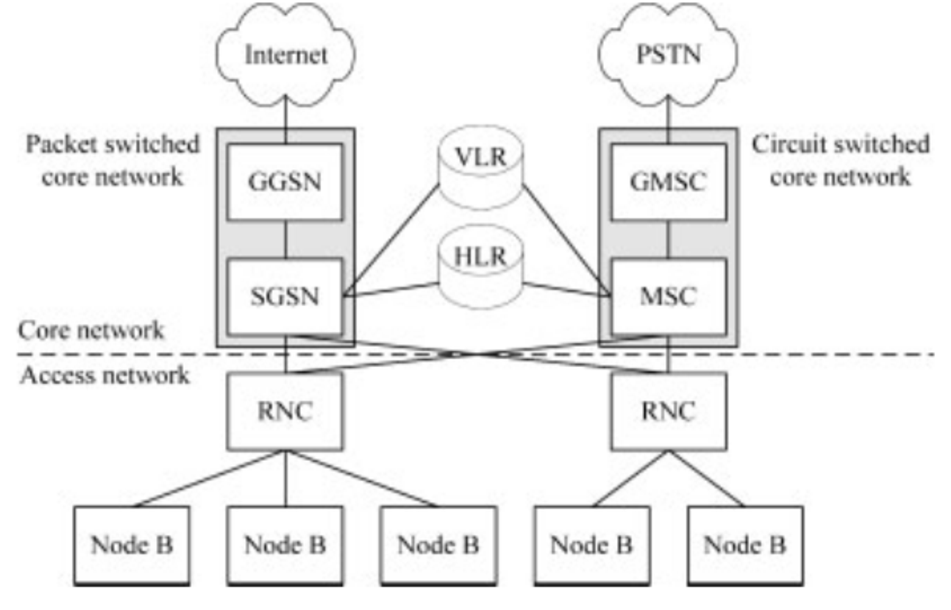
\includegraphics{UMTS.pdf}
\caption{Estructura básica de una infraestructura UMTS. Tomado de
@hilarie2008}
\end{figure}

Las estaciones bases (en este caso son los \emph{nodos B}) son usados
para trasmitir/recibir radiofrecuencia hacia/desde los usuarios móviles,
mientras que las RNC se ocupa de los recursos y la gestión de tráfico de
datos. El principal objetivo de la UTRAN (``\emph{UMTS Terrestrial Radio
Access Network}'') es hacer el enlace entre los usuarios móviles y el
núcleo red.

\paragraph{Planeación de Celda}\label{planeaciuxf3n-de-celda}

El autor \emph{Hitlarie}, descompone la planeación de las redes móviles
de manera modular, con el fin de reducir la complejidad y los divide en
los siguientes subproblemas:

\begin{itemize}
\item
  Subproblemas de planeación de celdas.
\item
  Subproblemas de planeación de red de acceso.
\item
  Subproblemas de planeación de núcleo de red.
\end{itemize}

La parte de los subproblemas que se necesita abordar con más detalle,
son los de planeación de celdas, ya que se asemeja más al enfoque que se
necesita en la planeación de redes inalámbricas de banda ancha; a
continuación, se describe dicho subproblema, así como algunos trabajos
que se han realizado.

\subparagraph{Subproblemas de planeación de
celdas}\label{subproblemas-de-planeaciuxf3n-de-celdas}

El problema inicial de planeación es cubrir todos los usuarios móviles
en un área determinada con el número mínimo de BSs. En la planeación de
celdas se encarga de resolver los siguientes ítems:

\begin{itemize}
\item
  Optimizar el número de BSs.
\item
  Mejor localización para instalar BSs.
\item
  Escoger el tipo o modelo de BSs.
\item
  Configuración (altura, orientación, potencia, etc).
\item
  Asignación de usuarios móviles a la BS.
\end{itemize}

Los problemas de planeación pueden variar dependiendo en la planeación
de red objetivo. Usualmente, en la planeación de red se requiere:

\begin{itemize}
\item
  Minimizar los costos de la red.
\item
  Maximizar la calidad de la señal.
\item
  Maximizar el área de cobertura.
\end{itemize}

Sin embargo, esto puede ser contradictorio, ya que, por ejemplo, si se
quiere maximizar la cobertura se necesitarán desplegar más BSs y esto
por supuesto, aumentara los costos. Al principio, la planeación de redes
inalámbricas se realizaba teniendo en cuenta la predicción de la señal,
sin embargo, en las redes UMTS, la planeación de radio no puede ser solo
basado en la predicción de la señal, sino que se deben tener en cuenta
la distribución de tráfico. En esta parte aparece gran cantidad de
literatura del autor Amaldi, en {[}@amaldi2003{]}, el autor
contextualiza que en la planeación de radio en el Sistema Global para
las Comunicaciones Móviles GSM (``\emph{Global System for Mobile
communications}'') se realizaba en dos fases, la fase de planeación de
cobertura donde se define la mejor localización de las BSs teniendo en
cuenta los modelos de propagación y la fase de planeación de frecuencia,
que define el número de canales para cada BS teniendo en cuenta la
calidad de la señal de interferencia de radio SIR
(``\emph{Signal-to-Interference Ratio}'').

Sin embargo, teniendo en cuenta el Acceso Múltiple por División de
Código de Banda Ancha W-CDMA (``\emph{Wideband Code Division Multiple
Access}''), esto ya no se puede realizar en estas dos fases, debido a
que el ancho de banda es compartido por todas las conexiones activas y
no por la frecuencia asignada, así como también el área de cobertura de
cada BS es afectada por la cantidad de tráfico.

Para la planeación de celdas, se tiene en cuenta los parámetros de
calidad de la SIR, en el cual se define una SIR mínima, el cual depende
de la potencia recibida; Esta depende de la potencia trasmitida y las
atenuaciones de señal en la propagación, por ende la potencia trasmitida
se puede ajustar para minimizar la interferencia, aquí aparece un
concepto importante, el cual es el control de potencia PC (``\emph{power
control}''), en donde se ajusta la potencia de trasmisión para cumplir
dos objetivos, la potencia objetivo recibida \(P_{tar}\) y la SIR
objetivo \(SIR_{tar}\). En este articulo \emph{Amaldi} propone un modelo
de programación matemática, que ayuda en la decisión de planear redes
móviles, teniendo en cuenta la mejor localización y configuración de las
BSs, teniendo en cuenta el modelo de propagación \emph{Hata}, donde se
ajusta el PC y este a su vez es probado con un algoritmo aleatorio
voraz, el cual añade o remueve BSs de la topología; En este artículo se
describe el rendimiento de esta solución dando resultados óptimos y
también demuestra que este problema es un problema típico de NP-hard.
Este trabajo se resalta por ser pionero en la planeación de celdas.

En la planeación de redes, a menudo se utiliza la optimización de varios
objetivos, más conocido como optimización multiobjetivo, el cual es
diferente de una optimización simple , puesto que aquí solo importa
optimizar un parámetro, dando como resultado el mejor diseño o la mejor
optimización, teniendo en cuenta un máximo o un mínimo global que
dependerá del objetivo de la optimización (maximizar o minimizar), sin
embargo, en la optimización multiobjetivo existe más de una solución
óptima con respecto a todos los objetivos; aquí, el objetivo consiste en
encontrar un óptimo de Pareto, el cual nos dice que una solución es
óptima cuando no existe otra solución tal que mejore en un objetivo sin
empeorar al menos uno de los otros.

Como se ha visto anteriormente, en la planeación se pueden abordar
diferentes objetivos (lugar de instalación de BS, configuración, altura,
potencia, etc.), sin embargo, al momento de planificar la red, atacar
todos los problemas al tiempo es un problema complejo, por esto, se han
venido implementando algoritmos multiobjetivo, generalmente para estos
casos se han venido desarrollando algoritmos genéticos AG, en el trabajo
de (@raisanen2005), los autores recolectan cuatro estados del arte de
algoritmos genéticos multiobjetivo, donde los ponen a prueba para
planificar una red aumentando la cobertura teniendo en cuenta los costos
y los comparan teniendo en cuenta su desempeño en ciertas pruebas
sintetizadas; los autores toman como referencia los algoritmos:
\textbf{SPEA2}, \textbf{NSGAII}, \textbf{PGSA} y \textbf{SEAMO}. A
continuación, se hará una breve descripción de cada uno.

\begin{itemize}
\tightlist
\item
  \textbf{SPEA2} (\emph{The Strength Pareto Evolutionary Algorithm
  version II})
\end{itemize}

La población inicial es sometida a una función de adecuación (``Fitness
Function''), donde se escoge el valor individual más apto o el más
``\emph{fit}'' de la unión del archivo y la población hija. El valor de
la función de adecuación está dado por la suma de dos partes: cuantas
soluciones domina (``\emph{raw fitness}'') y la \emph{densidad
estimada}, el cual es la proximidad de otras soluciones en el espacio
objetivo. Cada generación \(n\) es guardada en el archivo, en donde es
de nuevo aplicado el operador a la nueva generación; Este proceso se
repite hasta terminar el proceso.

\begin{itemize}
\tightlist
\item
  \textbf{NSGA II}
\end{itemize}

El individuo más apto está determinado por la unión del archivo y la
población hijo, determinado por mecanismos de clasificación compuesto de
dos partes. La primera parte está compuesta al determinar la capa de
soluciones que no son dominadas, es decir, las que están más cerca al
frente de pareto. La segunda parte es una medida de dispersión,
determinada por la distancia de hacinamiento crowding distance), el cual
se escogerá el que tenga menor hacinamiento, puesto que esto significa
que tendrá más población cubierta y la solución será más diversificada.
Este proceso se repetirá \(n\) repeticiones, guardando el valor de los
dos resultados y repitiendo lo mismo con las nuevas generaciones, hasta
que el algoritmo finalice.

\begin{itemize}
\tightlist
\item
  \textbf{PESA} (\emph{The Pareto Envelope-based Selection Algorithm})
\end{itemize}

A diferencia de los dos algoritmos anteriores, el \emph{PESA} no tiene
un tamaño de archivo fijo y solo permite que las soluciones no dominadas
sean miembros, por ende, es más limitado. Si el archivo excede el tamaño
de \(n\) soluciones, un factor de compresión o factor \emph{squeeze} ,
es calculado para todos los miembros del archivo. El factor de
compresión es el total de miembros en una subregión en una cuadricula
(las que están en el espacio de búsqueda, dentro de la subregión). El
factor de compresión más alto es el que tenga más vecinos locales en una
solución. Los miembros aleatorios de la región de la cuadrícula con el
factor de compresión más alto se eliminan hasta que se reduce el tamaño
del archivo a \(n\). Los operadores genéticos son aplicados en los
miembros del archivo a una nueva población hijo. Este proceso se repite
hasta la finalización.

\begin{itemize}
\tightlist
\item
  \textbf{SEAMO} (\emph{Simple Evolutionary Algorithm for
  Multi-objective Optimization})
\end{itemize}

La principal diferencia entre SEAMO y otro algoritmo, es que este es de
estado estable y solo mantiene una población (de un tamaño constante
\(n\)). La principal ventaja del algoritmo SEAMO es su simplicidad, el
cual usa la disposición de todos los mecanismos de selección basado en
fitness o rango. El avance de la búsqueda está definido por tres simples
reglas:

\begin{itemize}
\item
  los padres solo son remplazados por su propia descendencia.
\item
  Las poblaciones duplicadas son eliminadas.
\item
  La descendencia solo puede reemplazar a los padres si es superior:
  elitismo.
\end{itemize}

Los operadores genéticos se aplican a cada padre para formar un nuevo
hijo, que se considera para la sustitución en la población de padres
según las tres reglas. Este proceso se repite hasta la terminación.

El aspecto clave de este marco es un decodificador que utiliza un orden
de ubicaciones de sitios candidatos para construir una celda. En este
trabajo se concluyó que los algoritmos son similares en sus resultados
en términos reales, sin embargo, se encuentran algunas diferencias, el
\textbf{NGSA-II} y \textbf{SPEA2}, tienen resultados similares en cuanto
al rendimiento, el algoritmo \textbf{PESA} generalmente obtiene
ligeramente una baja calidad en el conjunto de soluciones, pero en
cuanto a la velocidad de convergencia y distribución de soluciones tiene
el mejor desempeño. En cuanto a \textbf{SEAMO}, se destaca por su
simplicidad, su elegancia conceptual, su fácil implementación y su
velocidad de ejecución, pero su simplicidad impide tener calidad en
cuanto a la distribución de las soluciones obtenidas y en el bajo
rendimiento en los factores medidos en el desarrollo del test. Para
finalizar el trabajo, los autores determinaron que el algoritmo
\textbf{NSGA-II} tiene el mejor rendimiento, siendo el que mejor se
podría implementar en la planeación de celdas ya que obtuvo los mejores
resultados de calidad en las soluciones obtenidas.

\subsubsection{Redes WiMAX}\label{redes-wimax}

En la planeación de celda, se han realizado trabajos con la tecnología
802.16e o WiMax; el autor (@gordejuela2009), presenta un marco de
referencia de optimización multiobjetivo que resuelve uno de los
principales problemas dentro del diseño inicial de redes de acceso
móvil, el cual es encontrar el mejor sitio de instalación de BSs dentro
de un conjunto de lugares posibles.

La forma en que le autor trabaja la planeación de la red, consiste en
que primero se realiza una predicción de la señal; aquí se tiene en
cuenta el tráfico de diferentes sitios candidatos posicionados
aleatoriamente en diferentes áreas geográficas, en esta fase evidencia
las densidades de tráfico entre áreas rurales y áreas urbanas. Una vez
se ha definido este modelo de tráfico, para realizar las funciones de
costos, el autor realiza una función de costos en la cual tiene en
cuenta el punto de equilibrio entre los diferentes factores que se
presentan en el diseño de una red, los cuales son:

\begin{itemize}
\item
  Área de cobertura.
\item
  Interferencia.
\item
  Rendimiento.
\item
  Rentabilidad de la operación de la red.
\item
  Equipamiento y otros costos.
\end{itemize}

La función de costos está dividida en dos partes, una consiste en una
función que tiene en cuenta los parámetros técnicos de rendimiento que
debe tener la red, como lo son penalizada con diferentes parámetros de
requerimientos que debe tener la red como son ancho de banda para
establecer videoconferencias, Voz IP, servicios en la red, etc. Calidad
de servicios QoS que deben tener los usuarios, entre otros. La otra
función de costos está contemplada por todos los parámetros de
rentabilidad que debe tener la red, para que la solución sea adecuada
para los proveedores de internet, en esta se tiene en cuenta la
rentabilidad de la red menos los costos de funcionamiento.

Una vez calculado estas funciones de costos, el paso a seguir es
realizar la optimización multiobjetivo de los parámetros anteriormente
analizados, esto se hace mediante el marco de referencia, en donde se va
realizando la simulación de la red con la herramienta de planeación
\emph{ForsK's Atoll}, donde posteriormente se va a realizar una técnica
de optimización con el algoritmo búsqueda tabú, donde el autor, modifica
el algoritmo para buscar la solución multiobjetivo, una vez realizado
esto, se van graficando las soluciones, con el fin de mostrarlas en el
óptimo de Pareto. Este procedimiento de realiza n veces, donde en cada
iteración, se realiza la técnica de optimización y se hace el ajuste
correspondiente a la solución, donde se vuelve a simular, esto hace
hasta encontrar una solución óptima.

En el trabajo de \emph{Gordejuela}, se realizó la implementación de este
marco de referencia de optimización multiobjetivo, donde se tuvo en
cuenta como criterio de planeación una cobertura basada en QoS, lograr
reducir al mínimo la interferencia y los costos de ubicar un conjunto de
20 BSs, luego se muestran los resultados de 600 iteraciones y se
demuestra que el maco de referencia a contribuido a un mejor resultado
con respecto a la solución sin planeación y que además tiene en cuenta
factores económicos que se pueden ajustar según las necesidades del
proveedor de la red, dando como resultado una herramienta de
optimización flexible y ofreciendo en este caso una comprensión
detallada de cómo se puede hacer la planeación optima utilizando redes
WiMax.

\subsubsection{Redes BWA en zonas
Rurales}\label{redes-bwa-en-zonas-rurales}

Prestar servicios de banda ancha en zonas rurales requiere de sistemas
de planeación dado que el acceso a estas zonas apartadas requiere
inversión en infraestructura para desplegar la topología física de la
red. Además, el desarrollo de las telecomunicaciones de banda ancha en
zonas rurales se enfrenta a numerosos desafíos dentro del ecosistema de
las telecomunicaciones de banda ancha, entre ellos se encuentran:

\begin{itemize}
\item
  Los gobiernos: Perspectiva política, jurídica y reglamentaria
\item
  Los reguladores: Políticas para el despliegue de infraestructura en
  zonas distantes
\item
  Los proveedores de servicios de telecomunicaciones: La inversión en
  telecomunicaciones rurales debe garantizar un negocio sostenible y
  viable
\item
  Los fabricantes de equipos de cliente (CPE): Costo de los equipos
\item
  Los consumidores: Costo elevado de los servicios, dificultad de acceso
  y disponibilidad, menor nivel de alfabetización tecnológica lo que
  imposibilita usar los servicios disponibles.
\end{itemize}

En la planeación de redes inalámbricas en áreas rurales, destacan los
autores (Sen, Bernardi, Rios), cada uno de ellos propone una planeación
de redes teniendo en cuenta su país de origen y priorizando las
necesidades, requisitos y restricciones que se tienen en cada uno de
ellos.

Con el objetivo de reducir la brecha digital, autores
{[}@bernardi2012{]},{[}@maseratti2011{]},{[}@sen{]} han propuesto como
solución la planeación y despliegue de redes de banda ancha inalámbrica
en zonas rurales; considerando las condiciones locales, como la
ubicación geográfica, el bienestar económico de la comunidad, el tipo de
entorno rural o urbano y el relieve del terreno, puede identificarse un
conjunto de posibles soluciones para prestar accesos de banda ancha, y
que van, entre otros, desde sistemas de cable a sistemas inalámbricos
fijos, sistemas satelitales o de enlaces de microondas, sistemas ADSL y
tecnologías móviles. A su vez, se destacan algunos trabajos de
planeación de redes BWA, los cuales se desarrollan en países con
marcadas diferencias de índices de desarrollo humano y el porcentaje de
población que vive en áreas rurales; se habla entonces de Reino Unido,
un país desarrollado donde el 17\% de la población vive en área rurales
y la India, un país en vía de desarrollo, donde el 66\% de la población
vive en áreas rurales.

\paragraph{Redes BWA en la India}\label{redes-bwa-en-la-india}

\textbf{Ubicación de la red}:

El autor \emph{Sen} se enfoca específicamente en la planeación de redes
de banda ancha en áreas rurales, en su tesis {[}@sen{]} trabaja sobre
una red desplegada en el distrito de Andhra del Oeste de Godavari
Pradesh ubicado en la India.

\textbf{Población a quién va dirigido:}

La India es un país donde la mayoría de la población vive en áreas
rurales (66\% según el Banco Mundial) y esta hace parte de la brecha
digital, esto se resuelve dando conectividad a todas las aldeas y
pueblos. Lograr esto expandiendo la red actual de telefónia fija en
zonas rurales no es factible teniendo en cuenta los costos elevados de
la instalación de la infraestructura inicial, sin embargo, este caso no
ocurre en la telefonía móvil, donde la demanda de usuarios es más densa
y por ende se considera un modelo de negocio, puesto que se retribuye la
inversión teniendo en cuenta la cantidad de usuarios dispuestos a pagar
por este servicio.

\textbf{Problemática:}

El problema radica en el hecho de que las zonas rurales tienen baja
densidad de usuarios y grandes distancias entre grupos de usuarios, esto
conlleva a que compañías de telecomunicaciones o proveedores de Internet
(ISP) vean poco atractiva la inversión en estos lugares debido al costo
inicial de infraestructura y despliegue de la red y bajo retorno de su
inversión.

\textbf{Causas:}

\begin{itemize}
\tightlist
\item
  Costo elevado de la expansión de la red telefónica fija
\item
  No es un modelo de negocio debido al bajo retorno de la inversión
\item
  Baja densidad de usuarios
\item
  Costo de infraestructura
\end{itemize}

\textbf{Solución:}

Por consiguiente, el autor propone la planeación de la topología de una
red inalámbrica con el uso de la tecnología 802.11, puesto que permite
una buena solución teniendo en cuenta su gran aceptabilidad,
principalmente por su bajo costo. Por ende, esta tecnología se ha
presentado como una opción de económica y efectiva para cubrir largas
distancias, ya que permite que zonas muy amplias puedan conectarse a un
nodo de línea terrestre con conectividad a Internet de forma cableada
(como fibra óptica) por medio de enlaces inalámbricos. Cada enlace
inalámbrico corresponde a una antena en una torre instalada en cada
pueblo, los cuales deben tener línea de vista \emph{L.O.S.} (\emph{Line
Of Sight}).

Para la formulación en la construcción de una topología que permita el
desempeño de la red, se estipulan de tres principales restricciones:

\begin{enumerate}
\def\labelenumi{\arabic{enumi}.}
\item
  Restricción de rendimiento: Capacidad de carga y descarga por cada
  nodo o pueblo que en el caso de la red en que se realizó el trabajo,
  se establecido que en cada nodo se tuviera un ancho de banda mínimo de
  384 Kps .
\item
  Restricción de Potencia: Se refiere al límite superior de la Potencia
  Isotrópica Irradiado (PIRE) en cada transmisor y el límite inferior de
  potencia recibida en el receptor (sensibilidad del receptor).
\item
  Restricción de interferencia: La señal recibida debe ser mayor al
  umbral de interferencia.
\end{enumerate}

El problema de la planeación es resuelto teniendo en cuenta una serie de
dependencias, los cuales están mostradas en la \emph{figura 2}. A
continuación se explicarán cada una de estas dependencias:

\begin{itemize}
\tightlist
\item
  La tasa de transferencia de datos depende de la MAC
\end{itemize}

El rendimiento requerido se logra dependiendo del protocolo MAC que se
esté implementando, en este caso, el autor propone utilizar el protocolo
de capa de Enlace de Datos 2P, puesto que en comparación con los
protocolos más utilizados como TDMA y CSMA/CA, este tiene una capacidad
de datos más elevada.

\begin{itemize}
\tightlist
\item
  La velocidad de transmisión depende del diseño físico de la red
\end{itemize}

El rendimiento depende del tipo de enlace, Punto a Punto (PTP) ó Punto
Multipunto (PMP), puesto que si es PTP se usa todo el rendimiento
permitido por la MAC, en cambio sí es PMP el rendimiento permitido por
la MAC se divide entre los enlaces que están conectados, de esta manera
el protocolo de enlace de todos tendrá que conmutar entre los enlaces
existentes reduciendo el rendimiento del protocolo MAC.

\begin{itemize}
\tightlist
\item
  La potencia de trasmisión depende del tamaño del enlace
\end{itemize}

La señal trasmitida tendrá una degradación en su intensidad, dependiendo
de la distancia del enlace. Cada antena tiene una ganancia especifica el
cual es la relación de densidad de energía que radia en una dirección
especifica.

\begin{itemize}
\tightlist
\item
  La MAC depende de la potencia de trasmisión
\end{itemize}

Esto es específicamente para el protocolo MAC 2P, en el que múltiples
enlaces pueden operar simultáneamente. La operación simultánea de
múltiples enlaces requiere que se asegure que la relación de potencias
de la señal real y de la interferencia (SIR) sea mayor que un margen
especificado por el sistema.

\begin{itemize}
\tightlist
\item
  La Altura de la torre depende del tamaño del enlace
\end{itemize}

La formación de un enlace Wifi entre dos nodos distanciados está basada
en L.O.S. el cual debe tener despejado el 60\% de la curvatura de la
zona de Fresnel. El tamaño de la zona de Fresnel dependerá de la
distancia del enlace.

\begin{itemize}
\tightlist
\item
  Los costos de despliegue dependen de la altura de las torres
\end{itemize}

Los costos de despliegue dependen principalmente del tamaño de la torre
que se van a implementar. Los costos de la torre crecen linealmente con
la altura de la torre, así que en este punto se debe considerar que se
debe diseñar la topología de tal forma que la altura sea la mínima, esto
ahorrará los costos principales del despliegue de una red.

\begin{figure}
\centering
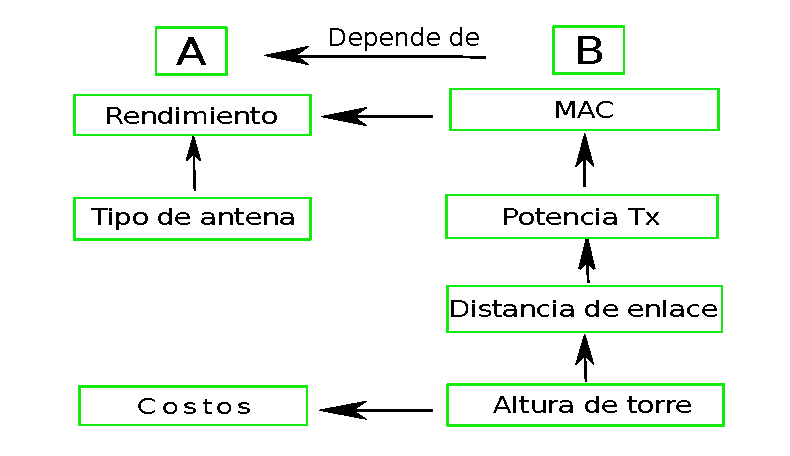
\includegraphics{dependencias.pdf}
\caption{Dependencias de requerimientos}
\end{figure}

\subparagraph{Consideraciones de diseño y enfoque de
solución}\label{consideraciones-de-diseuxf1o-y-enfoque-de-soluciuxf3n}

\begin{figure}
\centering
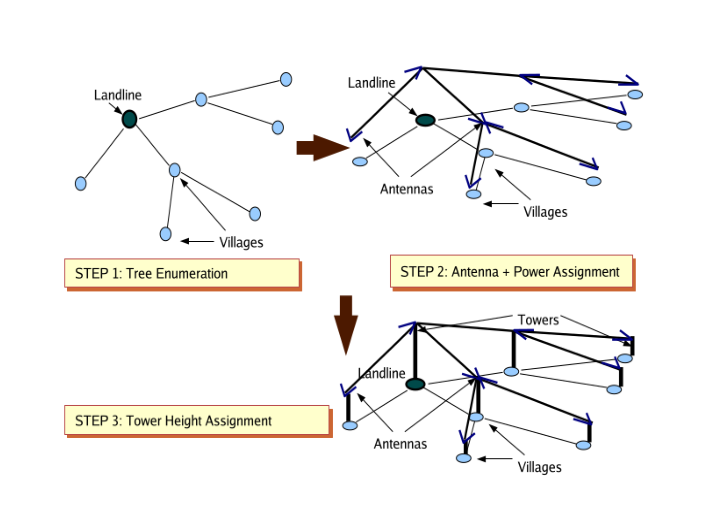
\includegraphics{sen.pdf}
\caption{Secuencia de pasos solución del problema de planeación en la
india}
\end{figure}

Una vez se ha visto como se divide el problema, el autor sugiere
resolver las dependencias con los siguientes pasos, el cual van a ser
explicados:

\begin{itemize}
\tightlist
\item
  \textbf{Topología de Búsqueda (TS)}:
\end{itemize}

Explorar el espacio de búsqueda para encontrar la topología de la red,
se hace uso del algoritmo Branch-and-bound (Algoritmo de ramificación y
límite), con ello se construye la topología de árbol, el cual va a dar
una topología inicial de la red.

\begin{itemize}
\tightlist
\item
  \textbf{Asignación de altura (HA)}:
\end{itemize}

Consiste en la altura óptima de las torres en las ubicaciones dadas una
vez que se ha formado la topología, para ello se utiliza un conjunto de
ecuaciones de programación lineal (LP), el cual se va a obtener la
altura que sea optima.

\begin{itemize}
\tightlist
\item
  \textbf{Asignación de Antena (AA)}:
\end{itemize}

Asignación apropiada de las antenas y sus respectivas orientaciones, se
desarrolla un algoritmo heurístico de tiempo complejo polinómico.

\begin{itemize}
\tightlist
\item
  \textbf{Asignación de Potencias (PA)}:
\end{itemize}

Proporcionar las potencias de transmisión en los radios del sistema
usando LP.

\textbf{Aporte final:}

Como aporte Sen entrega un algoritmo de planeación de redes en zonas
rurales y, una vez implementado, el autor en los resultados concluye que
se ahorró 22\% con respectos a una planeación sin ninguna técnica de
optimización.

\paragraph{Redes BWA en Escocia}\label{redes-bwa-en-escocia}

\textbf{Ubicación de la red:}

Bernardi diseñó e implementó \textbf{Tegola} un banco de pruebas que
proporciona internet a algunas comunidades remotas de Gran Bretaña, esta
red ha funcionado desde el año 2008 y ha comunicado a 20 comunidades en
toda Escocia. Esta red está situada en el noroeste de Escocia
comunicando comunidades rurales (principalmente costeras) en las
penínsulas de Glenelg y Knoydart en el continente británico hasta la
península de Sleat en la isla de Skye.

\textbf{Población a quién va dirigido:}

Gran Bretaña es un país desarrollado, comunmente llamado ``país del
primer mundo'' ya que su población en su mayoría vive en zonas urbanas,
sin embargo, el proyecto se enfoca en comunicar zonas rurales o
apartadas que no cuentan con acceso a internet de banda ancha (16,9\%
del total de la población).

\textbf{Problemática:}

La falta de herramientas de software para el diseño, gestión y
evaluación de redes de acceso inalámbrico de banda ancha han
obstaculizado su implementación generalizada a pesar de sus costos y
ventajas operativas sobre otras tecnologías de Acceso de banda ancha.

\textbf{Causas:}

\begin{itemize}
\tightlist
\item
  Costo de despliegue de ADSL
\item
  Bajo retorno de la inversión
\item
  Los usuarios viven lejos unos de otros
\item
  Costo de los equipos
\item
  No se puede accedes a software para comunicar pequeñas comunidades y
  pequeños WISP
\end{itemize}

Según \emph{Bernardi}, en las últimas décadas se ha incrementado la
conectividad de banda ancha, siendo la ADSL (del inglés Asymmetric
digital subscriber line) con más del 60\% de las conexiones de banda
ancha en países de la Organización para la Cooperación y el Desarrollo
Económicos es un organismo de cooperación internacional (OCDE); esto se
debe principalmente al éxito de la capitalización de ADSL debido al
éxito de la red de telefonía. Esta tecnología se caracteriza por que la
tasa de trasmisión máxima que puede alcanzar esta en función de la
distancia entre el usuario y la central telefónica, es decir, entre más
larga sea la distancia, la velocidad de trasmisión es más lenta, por
esta razón es comúnmente más utilizada en áreas metropolitanas debido a
que tiene más suscriptores y sea más efectivo retornar la inversión de
despliegue de una infraestructura. Esto es la principal causa de la
brecha digital que existe entre las áreas rurales y metropolitanas.

Pero \emph{Bernardi} expone el despliegue de una red Rural de Banda
Ancha (BWA) argumentando que la planeación ad-hoc no es una alternativa
de diseño eficiente para este tipo de redes, sin embargo, refiere que la
industria ofrece software para planeamiento de redes inalámbricas pero
estos no están disponibles ni son adecuados para comunicar pequeñas
comunidades y pequeños proveedores de servicio de Internet inalámbrico
(WISP) ; cabe resaltar que las BWA usan un modelo de dos niveles,
consistiendo en radioenlace Punto Multipunto (PMP) y Punto a Punto
(PTP), el primero enlazando la Antena de la torre a los diferentes
clientes y el segundo correspondiente al Backhaul.

\textbf{Solución :}

El Internet satelital se podría decir que es una alternativa de
conexión, puesto que está disponible prácticamente en cualquier parte y
es frecuentemente subsidiada en áreas remotas incomunicadas, sin
embargo, también tiene latencia de tiempo de ida y vuelta muy altos, lo
cual lo hace inadecuado para aplicaciones que consuman un ancho de banda
considerable, como es el caso de una videollamada (skape).

A través del planeamiento de red incremental \emph{Bernardi} desarrolla
un software denominado IncrEase cuyo enfoque es identificar la
estrategia de despliegue más económica para planear la red teniendo en
cuenta que los CPE (customer Premises Equipment) son la opción más
rentable para llegar a la población en zonas rurales.

Los proveedores de servicio de Internet inalámbrico implementan una
metodología de diseño para operar en escenarios rurales obteniendo
remuneración de su inversión, este consiste en planificar su crecimiento
ampliando su cobertura, tomando variables como:

\begin{itemize}
\item
  Limitar el alcance geográfico de los WISP:Para reducir los costos de
  operación.
\item
  Infraestructura de la red: En áreas rurales la fibra para el Backhaul
  no está disponible, por ello los WISP deben desplegar su propio
  Backhaul inalámbrico, aumentando los costos.
\item
  Cobertura de la red: El despliegue rural está basado en la cobertura
  más no en la capacidad.
\item
  Presupuesto ajustado: Los proveedores de Internet buscan obtener un
  retorno de su inversión desde su etapa de despliegue ya que las zonas
  rurales son entornos de baja rentabilidad.
\item
  Clientes agrupados: Proporcionar acceso a la red en sectores dónde
  haya más densidad de la población, para así captar más usuarios.
\end{itemize}

\emph{Bernardi} desarrolla un paquete de software con especial énfasis
en las regiones rurales y en desarrollo. Se resalta que abordó tres
desafíos técnicos en el contexto de redes de acceso inalámbrico de banda
ancha:

\begin{itemize}
\tightlist
\item
  Mapeo de Banda Ancha
\item
  Planeación de redes
\item
  Administración de redes
\end{itemize}

\textbf{Aporte:}

La contribución de \emph{Bernardi} es potenciar el negocio de los
pequeños proveedores de Internet inalámbrico (WISP) en zonas rurales a
través de un sistema de software, haciéndolo más eficiente reduciendo la
brecha digital, a través de la herramienta IncrEase.

Se desarrolla un software de código abierto IncrEase implementado como
una aplicación de escritorio multiplataforma en Java. IncrEase esta
basado en un GIS de software libre de la NASA World Wind Java y en una
base de datos gráfica Neo4J.

Para la implementación de IncrEase se toman tres fuentes:

\begin{itemize}
\tightlist
\item
  Demanda de la cobertura: Posibles usuarios de zonas rurales que no
  tienen acceso al servicio
\item
  Usuarios que fallaron en la etapa de instalación: Cobertura
  insuficiente
\item
  Reporte mesas de ayuda: Localización de los usuarios existentes
\end{itemize}

Además se obtienen otros datos de factores influyentes como la
disponibilidad DSL, la cobertura de red 3G y datos demográficos.
IncrEase a través de datos en forma de arreglo bidimensional cubre
regiones de interés y con ello obtiene mapas de calor (áreas de mayor
beneficio por la actualización de la red). En estos mapas a mayor calor
menor es la cobertura, una posible solución es la instalación de una
torre a partir de una lista de torres disponibles en esa área.

\begin{itemize}
\tightlist
\item
  \textbf{Modo de operación herramienta IncrEase}
\end{itemize}

Flujo de información de la herramienta

\begin{figure}
\centering
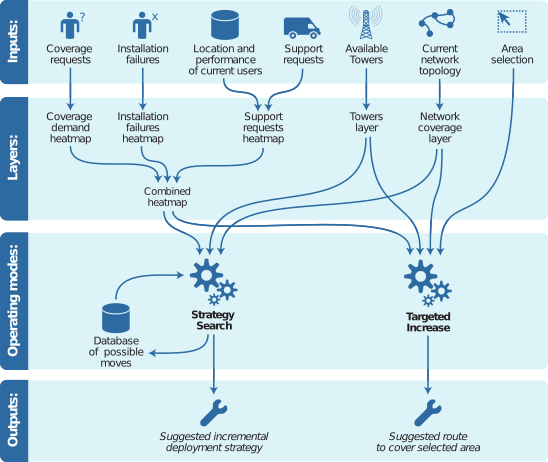
\includegraphics{figure4_1.png}
\caption{Ejemplo de flujo de informacion en la herramienta
\texttt{IncrEase}}
\end{figure}

\begin{itemize}
\item
  IncrEase Targeted: En este modo de operación el operador selecciona
  una región específica de cobertura, como parte de expansión de la red
\item
  Búsqueda Estratégica: Dónde la herramienta guía al operador para
  decidir el orden de despliegue de sitios de transmisión en el
  horizonte de corto o largo plazo basado en la rentabilidad esperada
\end{itemize}

\paragraph{Redes BWA en la región del Sumapaz
(Colombia)}\label{redes-bwa-en-la-regiuxf3n-del-sumapaz-colombia}

\textbf{Ubicación de la red:}

A nivel local, {[}@rios2015{]} propone una solución de construcción de
topología en redes rurales dentro de la realización Del Estudio De
Factibilidad, Socialización Y Capacitación, Para Implementación De
Infraestructuras De Voz Ip Y Comunicaciones Convergentes En La Región
Del Sumapaz '', del grupo de investigación GIGATT de la universidad de
Cundinamarca.

\textbf{Población a quién va dirigido:}

La región del Sumapaz es una de las quince provincias del Departamento
de Cundinamarca (Colombia), en ella se encuentra el páramo del Sumapaz,
el páramo más grande del mundo. Consta de 10 municipios con un 41\% de
población rural del total de la población referente al año 2011, el
énfasis del proyecto se plantea en la interconexión de estas zonas
apartadas.

\textbf{Problemática:}

Las adversas condiciones económicas y de acceso a las tecnologías de la
informa­ción, hacen que este proyecto busque evaluar la viabilidad y
conseguir alternativas asequibles de diseño e implementación de redes,
en este aspecto este trabajo pretende reducir los principales costos
involucrados en la implementación física de redes de comunicaciones
rurales

\textbf{Causas:}

\begin{itemize}
\tightlist
\item
  Costos de las torres
\item
  Baja densidad de la población
\item
  Bajo poder económico
\item
  Costos de infraestructura y equipos
\end{itemize}

\textbf{Solución:}

En el informe técnico ``Realización del estudio de factibilidad,
Socialización y Capacitación, para Implementación de Infraestructuras de
Voz Ip y Comisiones Convergentes en la Región del Sumapaz'' se plantea
la posibilidad de brindar acceso eficiente por medio de voz y video
llamadas a las zonas rurales de la región del Sumapaz, ofreciendo
cobertura a todas las localidades incluyendo las más vulnerables con una
calidad en el servicio coherente con el tipo de aplicación y con tarifas
acordes a la población, y paralelamente llevando a ellos servicios de
comunicaciones convergentes, haciendo de este un proyecto autosostenible
que coadyuve a la reducción de la brecha digital y permita el
aprovechamiento de los beneficios del programa de Mintic Vive Digital.

Hay que mencionar además que Ríos participó de forma activa en este
proyecto en el que la construcción de redes de comunicación rural
presenta particulares desafíos sobre todo en el costo que conlleva
establecerlas. Además refiere que un parámetro importante en el costo de
redes rurales es la construcción de torres que soporten las antenas a la
altura que permite establecer un buen enlace, debido a que este costo
domina otros costos de infraestructura como el atribuido a los equipos
de comunicación de el estandar IEEE 802.11 (WiFi), entonces el problema
principal se convierte en mantener costos mínimos en la construcción de
las torres de soporte para las antenas en cada nodo.

Ríos establece algunos factores principales en la planeación de la
construcción de la topología y son:

\begin{itemize}
\item
  Requerimientos de conectividad: Primero, es importante asegurar que la
  topología planteada permita la conexión de la totalidad de la red
\item
  Limitaciones físicas: Existen dos limitaciones físicas para la altura
  de las torres. Por ejemplo, existe una altura demasiada alta que
  representa un umbral para el cual los costos son prohibitivos y una
  altura mínima que limita el uso de torres tubulares
\item
  Naturaleza de la función de costos: Para alturas menores a 20m se
  suelen usar los mástiles económicos. Para alturas mayores, es
  necesario utilizar torres de acero más elaboradas, y por ende más
  caras, el costo de estas estructuras varía de manera casi lineal con
  la altura.
\item
  Condiciones sobre las alturas de las torres para establecer un enlace
  directo: Para ello se debe garantizar que la potencia de transmisión
  sea suficiente para superar las pérdidas por espacio libre en toda la
  distancia del enlace. También, se busca mantener la línea de vista
  despejada de toda obstrucción.
\end{itemize}

Dentro de este contexto y al igual que Sen, Bernardi, Maserati, expone
que el principal desafío es el costo que conlleva establecer redes en
zonas rurales, haciendo especial enfásis en el costo de construcción de
las torres que soportan las antenas, debido a que es el costo más grande
en comparación con los atribuidos a los equipos de comunicación.
Presenta los siguientes referentes:

\subparagraph{Topología}\label{topologuxeda}

Establece que las redes rurales mantienen una topología fija y se
realizan enlaces de larga distancia, sin embargo, al ser áreas
campestres existe una mayor cantidad de obstrucciones y acorde la
topografía varia la altura de los obstáculos.

\subparagraph{Costo de las torres}\label{costo-de-las-torres}

Para lograr obtener linea de vista entre los diferentes nodos es
necesario que las torres tengan una altura suficiente para superar los
obstáculos presentados en el terreno. Para la construcción de estas
torres establece dos tipos de materiales:

\begin{itemize}
\tightlist
\item
  Mástiles
\item
  Torres de acero ventadas
\end{itemize}

El costo de las torres, es proporcional a su altura y esta re­lacionado
con material de construcci6n, por ejemplo para un enlace de entre 7-8 Km
(distancias tfpicas) se necesitarfan torres de entre 30 m y 45 m con
costos de entre 25 y 38 millones de pesos colombianos. Este costo es de
varios ordenes de magnitud mayor que el de los equipos de
comunicaciones, de manera que el principal problema de construcción de
redes rurales radica en lograr una topología con el menor costo total de
las torres que soportan las antenas.

\textbf{Aporte:}

Para resolver el problema de la planeación el autor desarrolla un
algoritmo basado en (Panigrahi), dónde la solución resulta de dos
algoritmos TC-ALGO(G,c) y START-TC-ALGO(G,c), el primero determina el
valor de altura óptimo que permite obtener el mejor enlace dentro de un
grupo de enlaces vecinos a un nodo principal y el segundo permite
recorrer el grafo y ubicar el menor enlace o conjunto de enlaces que
representan el menor costo beneficio

\section{Capítulo 3. Diseño
metodológico}\label{capuxedtulo-3.-diseuxf1o-metodoluxf3gico}

\subsection{Generar el estado del arte de los algoritmos utilizados en
la planeación de redes inalámbricas que permitan identificar y
determinar los requerimientos del algoritmo que sugieran la mejor
estrategia de expansión de una
red}\label{generar-el-estado-del-arte-de-los-algoritmos-utilizados-en-la-planeaciuxf3n-de-redes-inaluxe1mbricas-que-permitan-identificar-y-determinar-los-requerimientos-del-algoritmo-que-sugieran-la-mejor-estrategia-de-expansiuxf3n-de-una-red}

En esta fase se indaga sobre las herramientas de planeación de redes
inalámbricas existentes con el propósito de recopilar información para
analizar y seleccionar la que más se adapte a la planeación de redes
inalámbricas de banda ancha en zonas rurales, en esta primera etapa se
realizan las siguientes actividades:

\subsubsection{\texorpdfstring{\textbf{Recolectar información de
planeación incremental de redes
inalámbricas}}{Recolectar información de planeación incremental de redes inalámbricas}}\label{recolectar-informaciuxf3n-de-planeaciuxf3n-incremental-de-redes-inaluxe1mbricas}

Este recurso se utiliza para registrar información relacionada con la
planeación de redes inalámbricas, se usó la técnica de recopilación
documental consultando libros, artículos de investigación en su mayoría
de la revista de Ingenieros Eléctricos y Electrónicos (IEEE), tesis,
informes y demás documentos que contribuyeran a proporcionar datos
enfocados en la temática central del proyecto. Lo que permitió obtener
un bajo costo considerando la gran cantidad de información que se
obtuvo, la bibliografía consultada es de característica técnica lo que
permitió lograr una dimensión histórica, social y tecnológica a través
del tiempo.

\subsubsection{\texorpdfstring{\textbf{Analizar la información
recopilada de redes inalámbricas enfocada a zonas
rurales}}{Analizar la información recopilada de redes inalámbricas enfocada a zonas rurales}}\label{analizar-la-informaciuxf3n-recopilada-de-redes-inaluxe1mbricas-enfocada-a-zonas-rurales}

Una vez se ha captado la información de planeación de redes se procede a
realizar su respectivo análisis, tabulando todos los documentos
encontrados,haciendo un rastreo y clasificación de los documentos,
detallando:

\begin{longtable}[]{@{}ll@{}}
\caption{Ficha bibliográfica para seleccionar los archivos de
estudio.}\tabularnewline
\toprule
Tipo de documento &\tabularnewline
Título &\tabularnewline
Año &\tabularnewline
URl &\tabularnewline
Temática central &\tabularnewline
Estado del arte y marco conceptual reseñado &\tabularnewline
Metodología &\tabularnewline
Resultados &\tabularnewline
\bottomrule
\end{longtable}

De este análisis de fuentes se encuentra que quince (15) son artículos
de investigación, cinco (5) son tesis y dos (2) son libros. De los
cuales se delimitan los temas a contextualizar, obteniendo los
siguientes:

\begin{itemize}
\tightlist
\item
  Brecha Digital
\item
  Redes Libres Comunitarias
\item
  Planeación de Redes Inalámbricas
\item
  Algoritmos utilizados en la planeación
\item
  Representación de la topología
\item
  Herramientas de manipulación de grafos
\item
  Planeación de redes móviles UMTS
\item
  Redes BWA en zonas rurales
\end{itemize}

Con ello se pudo establecer que los primeros seis puntos harían parte
del marco teórico y los dos siguientes pertenecerían al estado del arte,
esto como resultado de que el enfoque de esta investigación está
relacionado con la planeación de redes móviles y BWA en zonas rurales.

\subsubsection{\texorpdfstring{\textbf{Determinar la información que
cumpla con los requerimientos necesarios para diseñar el
algoritmo}}{Determinar la información que cumpla con los requerimientos necesarios para diseñar el algoritmo}}\label{determinar-la-informaciuxf3n-que-cumpla-con-los-requerimientos-necesarios-para-diseuxf1ar-el-algoritmo}

Acorde al análisis ejecutado en la actividad anterior se encontró que
los autores \emph{Bernardi}, \emph{Sen} y \emph{Milton} proporcionan la
información necesaria para diseñar el algoritmo. Dentro de los
requerimientos proporcionados se tienen:

\begin{itemize}
\tightlist
\item
  Topología de la red actual
\item
  Número de torres disponibles
\item
  Cobertura de la red, hace alusión al alcance geográfico
\item
  Altura de las torres
\item
  Zona de fresnel
\item
  Costo de despliegue de la red
\item
  Costo de la infraestructura y de los equipos
\item
  Algunos datos demográficos y económicos de la población
\end{itemize}

\subsubsection{\texorpdfstring{\textbf{Documentar el estado del
arte}}{Documentar el estado del arte}}\label{documentar-el-estado-del-arte}

Con toda la información analizada y los parámetros claros se documenta
el estado del arte realizando una comparación entre los tres autores
destacados mencionados con anterioridad. De ellos se establece

\begin{itemize}
\item
  Sen plantea su algoritmo en planear la red inalámbrica en zonas
  rurales de la India, se sabe que su contexto es social y rural
\item
  Bernardi desarrollo su software basado en Tegola, una red existente en
  Escocia, ampliando su cobertura a zonas rurales considerando el nivel
  lucrativo de la red enfocado en pequeños proveedores de internet
\item
  Milton por su parte, aplica el algoritmo de (Panigrahi) en la región
  del Sumapaz- Cundinamarca (Colombia) enfocando su idea en la
  interconexión de escuelas rurales añadiendo el costo de la
  construcción de la topología de la red.
\end{itemize}

En contexto, el estado del arte se puede estudiar en el capítulo 2 de
este Libro.

\subsection{Diseñar un algoritmo que permita identificar la mejor
estrategia de expansión de la red inalámbrica en zonas
rurales}\label{diseuxf1ar-un-algoritmo-que-permita-identificar-la-mejor-estrategia-de-expansiuxf3n-de-la-red-inaluxe1mbrica-en-zonas-rurales}

Partiendo del análisis e información recolectada se determinan los
parámetros necesarios para continuar con la etapa de diseño del
algoritmo para planear el crecimiento de una red inalámbrica en zonas
rurales.

Para el desarrollo del algoritmo que permite la creación de una
herramienta de planeación incremental de redes inalámbricas rurales, se
plantea el modelo cascada que en el desarrollo de software es un proceso
en el que todas las fases se realizan de forma secuencial, siguiendo un
flujo de ejecución de arriba hacia abajo como una cascada. Esto permite
hacer un fácil seguimiento del desarrollo del proyecto, realizando una
distribución de tareas y delimitando sus fases.

\begin{figure}
\centering
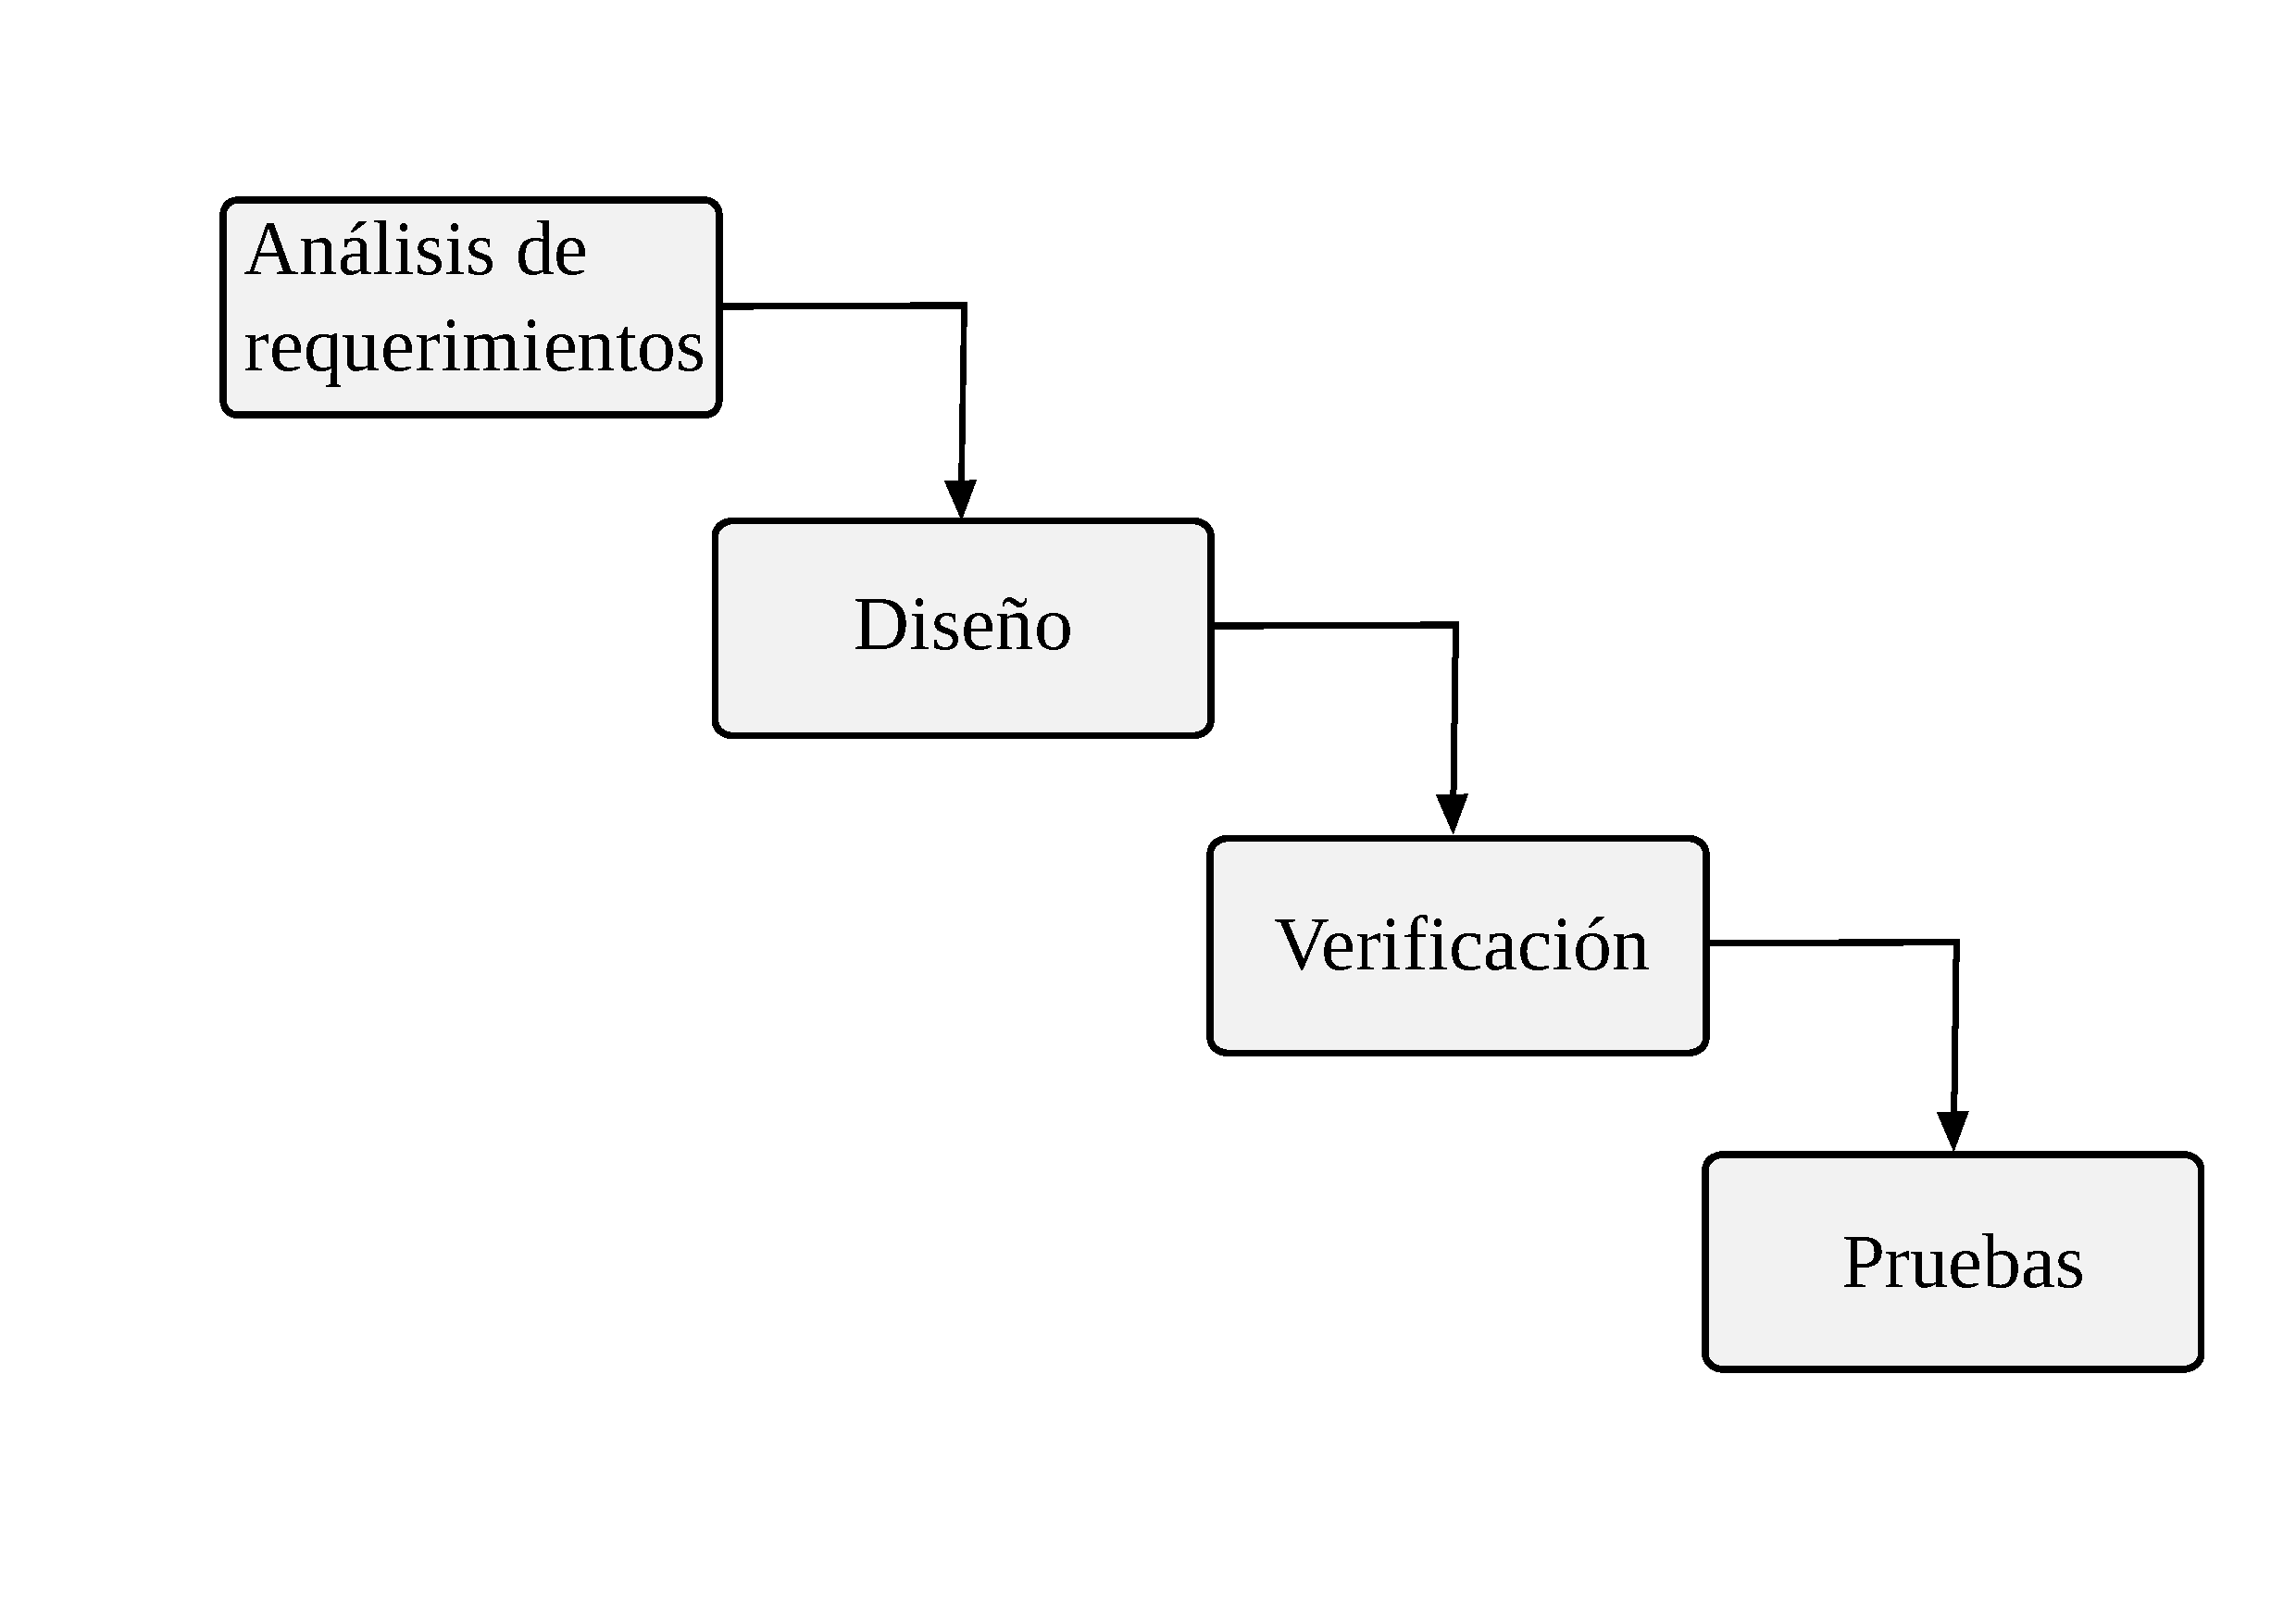
\includegraphics{metodologia.pdf}
\caption{Estructura metodología cascada}
\end{figure}

\subsubsection{Análisis de
requerimientos}\label{anuxe1lisis-de-requerimientos}

Resolver la brecha digital que existe entre las áreas urbanas y las
áreas rurales requiere aumentar la conectividad a Internet, para
asegurar la conexión en áreas rurales es necesario realizar una
planeación de redes inalámbricas que permita diseñar una infraestructura
con un mínimo costo al momento de desplegar la red.

Los autores {[}@Sen{]}, {[}panagrahi2008{]} y {[}@rios2015{]}, proponen
que la altura de la torre constituye uno de los costos más importantes
dentro de la construcción de una infraestructura de red inalámbrica en
áreas rurales, por esta razón se va a trabajar la asignación de la
altura mínima en las torres de instalación.

Asignación de altura de torres

\emph{Sen} propone una heurística que sigue una secuencia de pasos
explicados anteriormente y entre estos resuelve el problema de encontrar
una solución de alturas optimas utilizando programación lineal (PL), sin
embargo, en {[}@panagrahi2008{]} se propone un algoritmo para asignar la
altura donde cita a {[}@Sen {]}, puesto que sigue el mismo enfoque de
reducir el coste de infraestructura de red en zonas rurales, sin
embargo, el autor \emph{Panigrahi} proponen los algoritmos TC-ALGO Y
START-TC-ALGO que mejora la heurística que propone \emph{Sen}.

A continuación de describe las ventajas que tienen los algoritmos de
\emph{Panagrahi} sobre la heurística propuesta por \emph{Sen}:

\begin{itemize}
\item
  En la heurística no es posible conocer el límite de posibilidades,
  mientras en los algoritmos se tiene un límite de respuesta en el peor
  de los casos.
\item
  En la heurística se propone solo un obstáculo en la mitad del enlace
  entre dos nodos, sin embargo, los algoritmos pueden encargarse de
  encontrar la respuesta optima de la altura de las torres teniendo en
  cuenta todos los obstáculos entre el enlace de dos nodos.
\item
  En la heurística se trabaja una función de costo lineal por cada
  torre, mientras que los algoritmos usan una función de costos más
  general.
\end{itemize}

En {[}@rios2015{]} se propone el diseño de una topología de
infraestructura de red inalámbrica en la Región del Sumapaz
implementando los algoritmos planteados en {[}@ panagrahi2008{]}, en
este trabajo se implementan estos algoritmos para proponer una topología
que conecten unos puntos propuestos, en donde puede ir conectada una
torre de antena con la mínima altura de nodos, creando una topología de
mínimo costo.

Una vez desplegada la red con el mínimo costo es necesario guiar a los
ISP en la expansión de la red, de tal manera que puedan retornar la
inversión del costo de despliegue, en {[}@bernardi2012{]}, propone una
herramienta que facilita la planeación incremental de la red en zonas
rurales, utilizando dos modos de operación, targeted IncrEase y Búsqueda
estratégica, el primero permite identificar las zonas que deben ser
cubiertas por la red con una prioridad más alta y el segundo permite
saber en qué lugares es más factible la inversión. Por lo anterior, y
acorde al contexto local de este proyecto, existen proveedores de
internet que operan en la región y necesitan una herramienta que les
permita saber dónde invertir y aumentar la conexión en zonas rurales,
por ello se toma los dos modos de operación propuestos por Bernardi.

Una vez determinado los algoritmos que resuelven los requerimientos, se
detallan los parámetros de entrada y salida de cada uno de los
algoritmos propuestos por los autores.

\paragraph{Definir los datos de entrada y salida del
algoritmo}\label{definir-los-datos-de-entrada-y-salida-del-algoritmo}

En esta sección se especifican las variables de entrada y salida de los
algoritmos, entonces se tiene que:

\begin{itemize}
\tightlist
\item
  \textbf{Algoritmo planteado por Sen}
\end{itemize}

\begin{longtable}[]{@{}l@{}}
\caption{Datos de entrada del algoritmo planteado por
Sen.}\tabularnewline
\toprule
\begin{minipage}[b]{0.97\columnwidth}\raggedright\strut
Datos de entrada\strut
\end{minipage}\tabularnewline
\midrule
\endfirsthead
\toprule
\begin{minipage}[b]{0.97\columnwidth}\raggedright\strut
Datos de entrada\strut
\end{minipage}\tabularnewline
\midrule
\endhead
\begin{minipage}[t]{0.97\columnwidth}\raggedright\strut
Enumeración de todos los árboles y para cada árbol (coordenadas de la
ubicación de las villas)\strut
\end{minipage}\tabularnewline
\begin{minipage}[t]{0.97\columnwidth}\raggedright\strut
Asignación de las antenas\strut
\end{minipage}\tabularnewline
\begin{minipage}[t]{0.97\columnwidth}\raggedright\strut
Asignación de los valores de potencia de las antenas\strut
\end{minipage}\tabularnewline
\begin{minipage}[t]{0.97\columnwidth}\raggedright\strut
Asignación de las alturas de las torres en todos los nodos\strut
\end{minipage}\tabularnewline
\bottomrule
\end{longtable}

\begin{longtable}[]{@{}l@{}}
\caption{Datos de salida del algoritmo propuesto por
Sen.}\tabularnewline
\toprule
\begin{minipage}[b]{0.97\columnwidth}\raggedright\strut
Datos de Salida\strut
\end{minipage}\tabularnewline
\midrule
\endfirsthead
\toprule
\begin{minipage}[b]{0.97\columnwidth}\raggedright\strut
Datos de Salida\strut
\end{minipage}\tabularnewline
\midrule
\endhead
\begin{minipage}[t]{0.97\columnwidth}\raggedright\strut
Topología de la red\strut
\end{minipage}\tabularnewline
\begin{minipage}[t]{0.97\columnwidth}\raggedright\strut
Costo del árbol generado en comparación con otro anteriormente generado,
de lo dos se guarda el de menor costo\strut
\end{minipage}\tabularnewline
\bottomrule
\end{longtable}

\begin{itemize}
\tightlist
\item
  \textbf{Algoritmo diseñado por Bernardi}
\end{itemize}

\begin{longtable}[]{@{}l@{}}
\caption{Parámetros de entrada del algoritmo de
Bernardi.}\tabularnewline
\toprule
Datos de entrada\tabularnewline
\midrule
\endfirsthead
\toprule
Datos de entrada\tabularnewline
\midrule
\endhead
Demanda de cobertura\tabularnewline
Instalaciones fallidas\tabularnewline
Ubicación y desempeño de los usuarios actuales\tabularnewline
Solicitud de soporte\tabularnewline
Torres disponibles\tabularnewline
Topología de red actual\tabularnewline
Área de selección\tabularnewline
\bottomrule
\end{longtable}

\begin{longtable}[]{@{}l@{}}
\caption{Datos de Salida del algoritmo de bernardi.}\tabularnewline
\toprule
Datos de salida\tabularnewline
\midrule
\endfirsthead
\toprule
Datos de salida\tabularnewline
\midrule
\endhead
Estrategia incremental de despliegue sugerido\tabularnewline
Ruta sugerida para cubrir el área seleccionada\tabularnewline
\bottomrule
\end{longtable}

Cabe resaltar que este paquete de software proporciona dos modos de
operación que se han mencionado con anterioridad:

\begin{itemize}
\item
  Búsqueda estrategica: Cuya salida es la primer fila de la tabla
  anterior
\item
  Targeted Increase: donde se sugiere una ruta al área seleccionada
\item
  \textbf{Algoritmo implementado por Rios}
\end{itemize}

Esta aplicación esta basada en \emph{Panigrahi}, dónde resulta la
solución en dos algoritmos, el primero TC-ALGO(G,c) y el segundo
START-TC-ALGO(G,c).

\begin{longtable}[]{@{}ll@{}}
\caption{Parametros de entrada y salida del primer algoritmo de la
aplicación, TC-ALGO (G,c)}\tabularnewline
\toprule
Datos de entrada TC-Algo(G,c) & Datos de Salida
TC-ALGO(G,c)\tabularnewline
\midrule
\endfirsthead
\toprule
Datos de entrada TC-Algo(G,c) & Datos de Salida
TC-ALGO(G,c)\tabularnewline
\midrule
\endhead
Grafo G(V,E) & Función de alturas h\tabularnewline
Función de costos &\tabularnewline
\bottomrule
\end{longtable}

\begin{longtable}[]{@{}ll@{}}
\caption{Datos de entrada y salida del segundo algoritmo START-TC-ALGO
(G,c).}\tabularnewline
\toprule
Datos de entrada START-TC-ALGO (G,c) & Datos de salida START-TC-ALGO
(G,c)\tabularnewline
\midrule
\endfirsthead
\toprule
Datos de entrada START-TC-ALGO (G,c) & Datos de salida START-TC-ALGO
(G,c)\tabularnewline
\midrule
\endhead
Grafo G(V,E) & relación costo beneficio \(r'\) best\tabularnewline
Función de alturas h & incremento de altura incr\tabularnewline
Nodo n &\tabularnewline
Incremento altura variación en v &\tabularnewline
\bottomrule
\end{longtable}

Ahora, con los tipos de datos de entrada y salida de los algoritmos
estudiados, se determinan los parámetros de entrada y salida del
algoritmo que se va a diseñar. Es decir, que el algoritmo que se va a
proponer surge de la implementación secuencial de los algoritmos vistos
con anterioridad, seleccionando las variables que contribuyen a resolver
el problema a nivel local.

\begin{itemize}
\tightlist
\item
  \textbf{Algoritmo propuesto (Datos de entrada y salida)}
\end{itemize}

\begin{longtable}[]{@{}l@{}}
\caption{Parámetros de entrada algoritmo propuesto}\tabularnewline
\toprule
Datos de entrada\tabularnewline
\midrule
\endfirsthead
\toprule
Datos de entrada\tabularnewline
\midrule
\endhead
Grafo topología de la red\tabularnewline
Asignación de antenas\tabularnewline
Función de costos\tabularnewline
TC-ALGO\tabularnewline
START-TC-ALGO\tabularnewline
Limitar el alcance geográfico\tabularnewline
Red Backhaul disponible\tabularnewline
Solicitudes de Cobertura\tabularnewline
Clientes agrupados\tabularnewline
\bottomrule
\end{longtable}

\begin{longtable}[]{@{}l@{}}
\caption{Salida del algoritmo}\tabularnewline
\toprule
Datos de salida\tabularnewline
\midrule
\endfirsthead
\toprule
Datos de salida\tabularnewline
\midrule
\endhead
Mejor topología de expansión de la red con el menor costo\tabularnewline
\bottomrule
\end{longtable}

\subsubsection{Determinar los requerimientos necesarios para ejecutar el
algoritmo}\label{determinar-los-requerimientos-necesarios-para-ejecutar-el-algoritmo}

El estándar IEEE 830-1998 para el SRS(en inglés) o ERS (Especificación
de requerimientos de software) es un conjunto de recomendaciones para la
especificación de los requerimiento o requisitos de software, basado en
este estándar se determina:

\begin{itemize}
\tightlist
\item
  \textbf{Requerimientos funcionales}
\end{itemize}

\begin{longtable}[]{@{}ll@{}}
\toprule
Identificador del requerimiento & Entrada 1\tabularnewline
\midrule
\endhead
Nombre del requerimiento & Cobertura\tabularnewline
Características & Ubicación de la red existente\tabularnewline
Descripción del requerimiento & Límite geográfico de la red
actual\tabularnewline
Requerimiento NO funcional &\tabularnewline
Prioridad del requerimiento & Alta\tabularnewline
\bottomrule
\end{longtable}

Table:

\begin{longtable}[]{@{}ll@{}}
\toprule
\begin{minipage}[b]{0.39\columnwidth}\raggedright\strut
Identificador del requerimiento\strut
\end{minipage} & \begin{minipage}[b]{0.50\columnwidth}\raggedright\strut
Entrada 2\strut
\end{minipage}\tabularnewline
\midrule
\endhead
\begin{minipage}[t]{0.39\columnwidth}\raggedright\strut
Nombre del requerimiento\strut
\end{minipage} & \begin{minipage}[t]{0.50\columnwidth}\raggedright\strut
Ubicación de los usuarios\strut
\end{minipage}\tabularnewline
\begin{minipage}[t]{0.39\columnwidth}\raggedright\strut
Características\strut
\end{minipage} & \begin{minipage}[t]{0.50\columnwidth}\raggedright\strut
Identificación de la ubicación geográfica de los usuarios\strut
\end{minipage}\tabularnewline
\begin{minipage}[t]{0.39\columnwidth}\raggedright\strut
Descripción del requerimiento\strut
\end{minipage} & \begin{minipage}[t]{0.50\columnwidth}\raggedright\strut
Detallar la localización geográfica de los usuarios para analizar la
topografía del terreno\strut
\end{minipage}\tabularnewline
\begin{minipage}[t]{0.39\columnwidth}\raggedright\strut
Requerimiento NO funcional\strut
\end{minipage} & \begin{minipage}[t]{0.50\columnwidth}\raggedright\strut
\strut
\end{minipage}\tabularnewline
\begin{minipage}[t]{0.39\columnwidth}\raggedright\strut
Prioridad del requerimiento\strut
\end{minipage} & \begin{minipage}[t]{0.50\columnwidth}\raggedright\strut
Alta\strut
\end{minipage}\tabularnewline
\bottomrule
\end{longtable}

Table:

\begin{longtable}[]{@{}ll@{}}
\toprule
\begin{minipage}[b]{0.39\columnwidth}\raggedright\strut
Identificador del requerimiento\strut
\end{minipage} & \begin{minipage}[b]{0.50\columnwidth}\raggedright\strut
Entrada 3\strut
\end{minipage}\tabularnewline
\midrule
\endhead
\begin{minipage}[t]{0.39\columnwidth}\raggedright\strut
Nombre del requerimiento\strut
\end{minipage} & \begin{minipage}[t]{0.50\columnwidth}\raggedright\strut
Torres disponibles\strut
\end{minipage}\tabularnewline
\begin{minipage}[t]{0.39\columnwidth}\raggedright\strut
Características\strut
\end{minipage} & \begin{minipage}[t]{0.50\columnwidth}\raggedright\strut
Obtener acceso a la ubicación de las torres\strut
\end{minipage}\tabularnewline
\begin{minipage}[t]{0.39\columnwidth}\raggedright\strut
Descripción del requerimiento\strut
\end{minipage} & \begin{minipage}[t]{0.50\columnwidth}\raggedright\strut
La ubicación espacial de las torres en el área de implementación de la
topología de la red, permite saber que torres o conjuntos de ellas se
pueden utilizar y así disminuir los costos de instalación\strut
\end{minipage}\tabularnewline
\begin{minipage}[t]{0.39\columnwidth}\raggedright\strut
Requerimiento NO funcional\strut
\end{minipage} & \begin{minipage}[t]{0.50\columnwidth}\raggedright\strut
\strut
\end{minipage}\tabularnewline
\begin{minipage}[t]{0.39\columnwidth}\raggedright\strut
Prioridad del requerimiento\strut
\end{minipage} & \begin{minipage}[t]{0.50\columnwidth}\raggedright\strut
Alta\strut
\end{minipage}\tabularnewline
\bottomrule
\end{longtable}

Table:

\begin{longtable}[]{@{}ll@{}}
\toprule
\begin{minipage}[b]{0.39\columnwidth}\raggedright\strut
Identificador del requerimiento\strut
\end{minipage} & \begin{minipage}[b]{0.50\columnwidth}\raggedright\strut
Entrada 4\strut
\end{minipage}\tabularnewline
\midrule
\endhead
\begin{minipage}[t]{0.39\columnwidth}\raggedright\strut
Nombre del requerimiento\strut
\end{minipage} & \begin{minipage}[t]{0.50\columnwidth}\raggedright\strut
Topología de la red\strut
\end{minipage}\tabularnewline
\begin{minipage}[t]{0.39\columnwidth}\raggedright\strut
Características\strut
\end{minipage} & \begin{minipage}[t]{0.50\columnwidth}\raggedright\strut
Obtener topología de la red existente y su ampliación\strut
\end{minipage}\tabularnewline
\begin{minipage}[t]{0.39\columnwidth}\raggedright\strut
\strut
\end{minipage}\tabularnewline
\begin{minipage}[t]{0.39\columnwidth}\raggedright\strut
Descripción del requerimiento\strut
\end{minipage} & \begin{minipage}[t]{0.50\columnwidth}\raggedright\strut
Diseñar a partir de la topología de la red existente una nueva topología
con el propósito de aumentar su cobertura y permitir que más usuarios
accedad a ella.\strut
\end{minipage}\tabularnewline
\begin{minipage}[t]{0.39\columnwidth}\raggedright\strut
Requerimiento NO funcional\strut
\end{minipage} & \begin{minipage}[t]{0.50\columnwidth}\raggedright\strut
\strut
\end{minipage}\tabularnewline
\begin{minipage}[t]{0.39\columnwidth}\raggedright\strut
Prioridad del requerimiento\strut
\end{minipage} & \begin{minipage}[t]{0.50\columnwidth}\raggedright\strut
Alta\strut
\end{minipage}\tabularnewline
\bottomrule
\end{longtable}

Table:

\begin{longtable}[]{@{}ll@{}}
\toprule
\begin{minipage}[b]{0.39\columnwidth}\raggedright\strut
Identificador del requerimiento\strut
\end{minipage} & \begin{minipage}[b]{0.50\columnwidth}\raggedright\strut
Entrada 5\strut
\end{minipage}\tabularnewline
\midrule
\endhead
\begin{minipage}[t]{0.39\columnwidth}\raggedright\strut
Nombre del requerimiento\strut
\end{minipage} & \begin{minipage}[t]{0.50\columnwidth}\raggedright\strut
Área de selección\strut
\end{minipage}\tabularnewline
\begin{minipage}[t]{0.39\columnwidth}\raggedright\strut
Características\strut
\end{minipage} & \begin{minipage}[t]{0.50\columnwidth}\raggedright\strut
Determinar la zona rural en dónde se realizará la expansión de la
red\strut
\end{minipage}\tabularnewline
\begin{minipage}[t]{0.39\columnwidth}\raggedright\strut
Descripción del requerimiento\strut
\end{minipage} & \begin{minipage}[t]{0.50\columnwidth}\raggedright\strut
Al seleccionar la ubicación geográfica dónde se aplicará el algoritmo se
analizarán las condiciones del terreno para la ubicación de las
torres\strut
\end{minipage}\tabularnewline
\begin{minipage}[t]{0.39\columnwidth}\raggedright\strut
Requerimiento NO funcional\strut
\end{minipage} & \begin{minipage}[t]{0.50\columnwidth}\raggedright\strut
\strut
\end{minipage}\tabularnewline
\begin{minipage}[t]{0.39\columnwidth}\raggedright\strut
Prioridad del requerimiento\strut
\end{minipage} & \begin{minipage}[t]{0.50\columnwidth}\raggedright\strut
Alta\strut
\end{minipage}\tabularnewline
\bottomrule
\end{longtable}

Table:

\begin{longtable}[]{@{}ll@{}}
\toprule
\begin{minipage}[b]{0.39\columnwidth}\raggedright\strut
Identificador del requerimiento\strut
\end{minipage} & \begin{minipage}[b]{0.50\columnwidth}\raggedright\strut
Entrada 6\strut
\end{minipage}\tabularnewline
\midrule
\endhead
\begin{minipage}[t]{0.39\columnwidth}\raggedright\strut
Nombre del requerimiento\strut
\end{minipage} & \begin{minipage}[t]{0.50\columnwidth}\raggedright\strut
Ingreso de los datos\strut
\end{minipage}\tabularnewline
\begin{minipage}[t]{0.39\columnwidth}\raggedright\strut
Características\strut
\end{minipage} & \begin{minipage}[t]{0.50\columnwidth}\raggedright\strut
Datos de entrada del algoritmo\strut
\end{minipage}\tabularnewline
\begin{minipage}[t]{0.39\columnwidth}\raggedright\strut
Descripción del requerimiento\strut
\end{minipage} & \begin{minipage}[t]{0.50\columnwidth}\raggedright\strut
Permite que los diseñadores del algoritmo ingresen las difernetes
variables o datos para el funconamiento del programa.\strut
\end{minipage}\tabularnewline
\begin{minipage}[t]{0.39\columnwidth}\raggedright\strut
Requerimiento NO funcional\strut
\end{minipage} & \begin{minipage}[t]{0.50\columnwidth}\raggedright\strut
\strut
\end{minipage}\tabularnewline
\begin{minipage}[t]{0.39\columnwidth}\raggedright\strut
Prioridad del requerimiento\strut
\end{minipage} & \begin{minipage}[t]{0.50\columnwidth}\raggedright\strut
Alta\strut
\end{minipage}\tabularnewline
\bottomrule
\end{longtable}

Table:

\begin{longtable}[]{@{}ll@{}}
\toprule
\begin{minipage}[b]{0.39\columnwidth}\raggedright\strut
Identificador del requerimiento\strut
\end{minipage} & \begin{minipage}[b]{0.50\columnwidth}\raggedright\strut
Entrada 7\strut
\end{minipage}\tabularnewline
\midrule
\endhead
\begin{minipage}[t]{0.39\columnwidth}\raggedright\strut
Nombre del requerimiento\strut
\end{minipage} & \begin{minipage}[t]{0.50\columnwidth}\raggedright\strut
Operaciones matemáticas\strut
\end{minipage}\tabularnewline
\begin{minipage}[t]{0.39\columnwidth}\raggedright\strut
Características\strut
\end{minipage} & \begin{minipage}[t]{0.50\columnwidth}\raggedright\strut
Procesos matemáticos para obtener una respuesta óptima\strut
\end{minipage}\tabularnewline
\begin{minipage}[t]{0.39\columnwidth}\raggedright\strut
Descripción del requerimiento\strut
\end{minipage} & \begin{minipage}[t]{0.50\columnwidth}\raggedright\strut
PLas operaciones matemáticas permiten al algoritmo brindar una respuesta
óptima sobre la ubicación de las torres en el lugar donde se expandirá
la red, esto conlleva a realizar calculos para que su implementación sea
de menor costo\strut
\end{minipage}\tabularnewline
\begin{minipage}[t]{0.39\columnwidth}\raggedright\strut
Requerimiento NO funcional\strut
\end{minipage} & \begin{minipage}[t]{0.50\columnwidth}\raggedright\strut
\strut
\end{minipage}\tabularnewline
\begin{minipage}[t]{0.39\columnwidth}\raggedright\strut
Prioridad del requerimiento\strut
\end{minipage} & \begin{minipage}[t]{0.50\columnwidth}\raggedright\strut
Alta\strut
\end{minipage}\tabularnewline
\bottomrule
\end{longtable}

Table:

\begin{itemize}
\tightlist
\item
  \textbf{Requerimientos NO funcionales}
\end{itemize}

\begin{longtable}[]{@{}ll@{}}
\toprule
\begin{minipage}[b]{0.39\columnwidth}\raggedright\strut
Identificador del requerimiento\strut
\end{minipage} & \begin{minipage}[b]{0.50\columnwidth}\raggedright\strut
INT01\strut
\end{minipage}\tabularnewline
\midrule
\endhead
\begin{minipage}[t]{0.39\columnwidth}\raggedright\strut
Nombre del requerimiento\strut
\end{minipage} & \begin{minipage}[t]{0.50\columnwidth}\raggedright\strut
Rápidez del algoritmo\strut
\end{minipage}\tabularnewline
\begin{minipage}[t]{0.39\columnwidth}\raggedright\strut
Características\strut
\end{minipage} & \begin{minipage}[t]{0.50\columnwidth}\raggedright\strut
Desempeño en la ejecución del algoritmo.\strut
\end{minipage}\tabularnewline
\begin{minipage}[t]{0.39\columnwidth}\raggedright\strut
Descripción del requerimiento\strut
\end{minipage} & \begin{minipage}[t]{0.50\columnwidth}\raggedright\strut
Evaluar el desempeño en velocidad de respuesta del algoritmo a los datos
de entrada ingresados por el diseñador\strut
\end{minipage}\tabularnewline
\begin{minipage}[t]{0.39\columnwidth}\raggedright\strut
Requerimiento NO funcional\strut
\end{minipage} & \begin{minipage}[t]{0.50\columnwidth}\raggedright\strut
\strut
\end{minipage}\tabularnewline
\begin{minipage}[t]{0.39\columnwidth}\raggedright\strut
Prioridad del requerimiento\strut
\end{minipage} & \begin{minipage}[t]{0.50\columnwidth}\raggedright\strut
Alta\strut
\end{minipage}\tabularnewline
\bottomrule
\end{longtable}

Table:

\begin{longtable}[]{@{}ll@{}}
\toprule
\begin{minipage}[b]{0.39\columnwidth}\raggedright\strut
Identificador del requerimiento\strut
\end{minipage} & \begin{minipage}[b]{0.50\columnwidth}\raggedright\strut
INT02\strut
\end{minipage}\tabularnewline
\midrule
\endhead
\begin{minipage}[t]{0.39\columnwidth}\raggedright\strut
Nombre del requerimiento\strut
\end{minipage} & \begin{minipage}[t]{0.50\columnwidth}\raggedright\strut
Requerimientos de procesamiento\strut
\end{minipage}\tabularnewline
\begin{minipage}[t]{0.39\columnwidth}\raggedright\strut
Características\strut
\end{minipage} & \begin{minipage}[t]{0.50\columnwidth}\raggedright\strut
Capacidad de la memoria del pc para procesar el algoritmo\strut
\end{minipage}\tabularnewline
\begin{minipage}[t]{0.39\columnwidth}\raggedright\strut
Descripción del requerimiento\strut
\end{minipage} & \begin{minipage}[t]{0.50\columnwidth}\raggedright\strut
Determinar cuanto espacio y memoria necesita el equipo para procesar y
ejecutar el algoritmo\strut
\end{minipage}\tabularnewline
\begin{minipage}[t]{0.39\columnwidth}\raggedright\strut
Requerimiento NO funcional\strut
\end{minipage} & \begin{minipage}[t]{0.50\columnwidth}\raggedright\strut
\strut
\end{minipage}\tabularnewline
\begin{minipage}[t]{0.39\columnwidth}\raggedright\strut
Prioridad del requerimiento\strut
\end{minipage} & \begin{minipage}[t]{0.50\columnwidth}\raggedright\strut
Alta\strut
\end{minipage}\tabularnewline
\bottomrule
\end{longtable}

Table:

\begin{longtable}[]{@{}ll@{}}
\toprule
\begin{minipage}[b]{0.39\columnwidth}\raggedright\strut
Identificador del requerimiento\strut
\end{minipage} & \begin{minipage}[b]{0.50\columnwidth}\raggedright\strut
INT03\strut
\end{minipage}\tabularnewline
\midrule
\endhead
\begin{minipage}[t]{0.39\columnwidth}\raggedright\strut
Nombre del requerimiento\strut
\end{minipage} & \begin{minipage}[t]{0.50\columnwidth}\raggedright\strut
Lenguaje de programación\strut
\end{minipage}\tabularnewline
\begin{minipage}[t]{0.39\columnwidth}\raggedright\strut
Características\strut
\end{minipage} & \begin{minipage}[t]{0.50\columnwidth}\raggedright\strut
Python\strut
\end{minipage}\tabularnewline
\begin{minipage}[t]{0.39\columnwidth}\raggedright\strut
Descripción del requerimiento\strut
\end{minipage} & \begin{minipage}[t]{0.50\columnwidth}\raggedright\strut
El algoritmo se desarrollará en el lenguaje de programación Python\strut
\end{minipage}\tabularnewline
\begin{minipage}[t]{0.39\columnwidth}\raggedright\strut
Requerimiento NO funcional\strut
\end{minipage} & \begin{minipage}[t]{0.50\columnwidth}\raggedright\strut
\strut
\end{minipage}\tabularnewline
\begin{minipage}[t]{0.39\columnwidth}\raggedright\strut
Prioridad del requerimiento\strut
\end{minipage} & \begin{minipage}[t]{0.50\columnwidth}\raggedright\strut
Alta\strut
\end{minipage}\tabularnewline
\bottomrule
\end{longtable}

Table:

\subsubsection{Diseño}\label{diseuxf1o}

\paragraph{Proponer el conjunto de operaciones secuenciales para la
realización del
Algoritmo}\label{proponer-el-conjunto-de-operaciones-secuenciales-para-la-realizaciuxf3n-del-algoritmo}

A partir de los tres algoritmos estudiados se plantea una nueva
propuesta para el planeamiento de redes inalámbricas en zonas
rurales.Para esto, se toman algunas características que contribuyen a
dar solución al problema local (expandir la red Libre de Bosachoque a la
región del Sumapaz), esto con el fin de generar un nuevo algoritmo que
permita dar conectividad a internet en zonas apartadas a un bajo costo.

Para proponer un nuevo algoritmo se establece:

\begin{enumerate}
\def\labelenumi{\arabic{enumi}.}
\tightlist
\item
  Parámetros de entrada
\item
  Planeación incremental
\item
  Planeación del costo mínimo
\item
  Salida: Obtener una respuesta de planeación de redes inalámbricas
  rurales económica
\end{enumerate}

En la siguiente figura se establece el diagrama sistémico del modo de
operación de la herramienta propuesta.

\begin{figure}
\centering
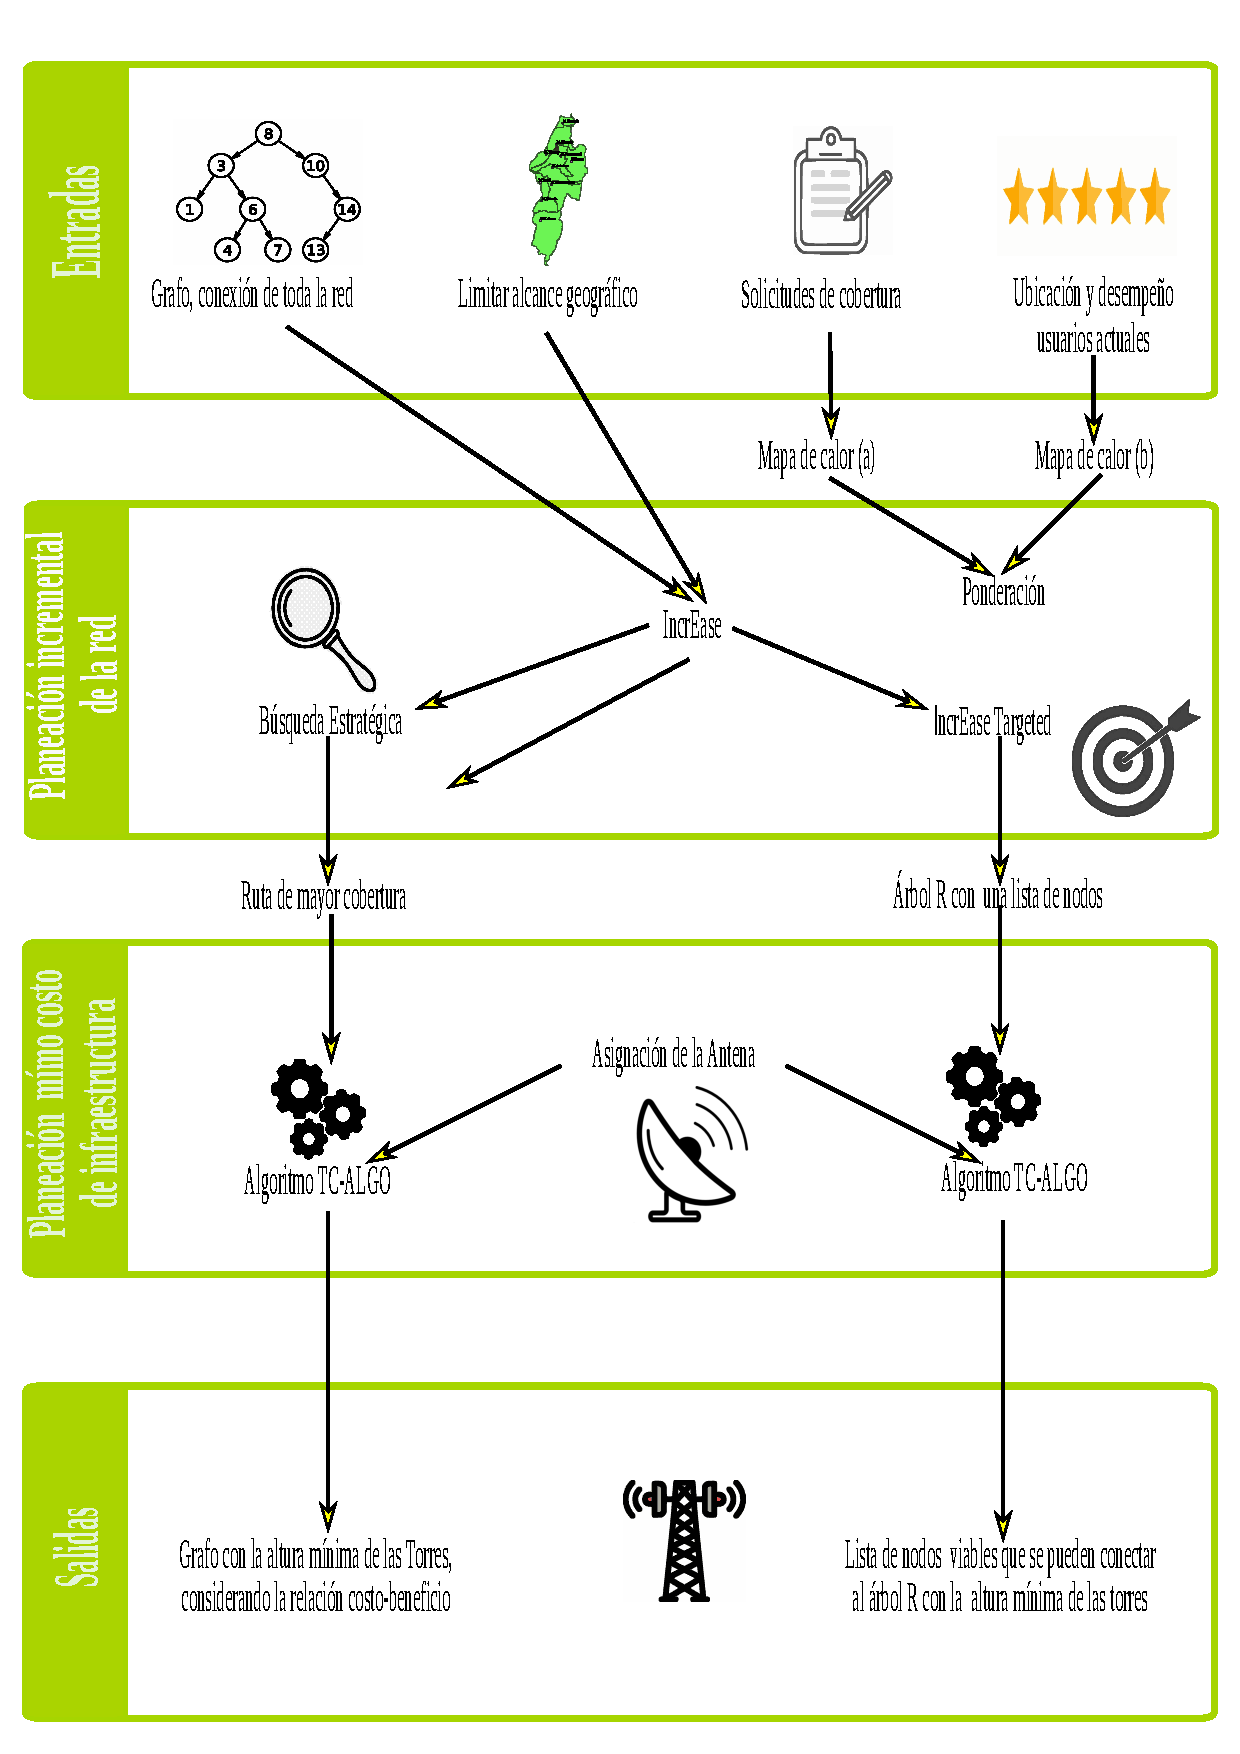
\includegraphics{Diagrama_sistemico.pdf}
\caption{Diagrama sistémico}
\end{figure}

\textbf{Descripción del proceso de operación del algoritmo propuesto}

\begin{enumerate}
\def\labelenumi{\arabic{enumi}.}
\tightlist
\item
  \textbf{Parámetros de entrada}
\end{enumerate}

\begin{itemize}
\item
  Grafo, conexión de toda la red: se ingresa un grafo con una topología
  propuesta dónde todos los nodos se encuentren conectados entre sí.
\item
  Limitar el alcance geográfico: Se delimita la región en dónde se desea
  expandir la red existente.
\item
  Solicitudes de cobertura: sectores o usuarios que desean adquirir el
  servicio de conectividad a Internet.
\end{itemize}

\begin{enumerate}
\def\labelenumi{\arabic{enumi}.}
\setcounter{enumi}{1}
\tightlist
\item
  \textbf{Planeación incremental de la red}
\end{enumerate}

\textbf{Mapas de calor}

Los mapas de calor son una herramienta visual que permite al usuario
identificar zonas en dónde se necesita con mayor prioridad brindar
conectividad a Internet. Entonces, a mayor concentración de color más
alta es la prioridad.

Para realizar estos mapas se utiliza la herramienta QGIS, que es un
cliente GIS de código abierto fácil de usar, donde se puede visualizar,
administrar, editar, analizar datos y componer mapas imprimibles.
Además, incluye una poderosa funcionalidad analítica a través de la
integración con GRASS, SAGA, Orfeo Toolbox , GDAL/OGR y muchos otros
proveedores de algoritmos.

Se consideran dos fuentes de información, de cada fuente se genera un
mapa de calor diferente.

\begin{itemize}
\item
  Mapa de calor de las solicitudes de cobertura: sugiere los lugares en
  los que se encuentra mayor cantidad de usuarios que solicitan el
  servicio.
\item
  Mapa de calor de la ubicación y desempeño de los usuarios actuales:
  Permite saber la ubicación de los usuarios que hacen parte de la red
  actual y el nivel de funcionamiento de estos nodos.
\end{itemize}

Una vez se han obtenido los mapas de calor se hace la unión de los tres
a fin de determinar que lugares se deben cubrir con mayor prioridad,
teniendo en cuenta la relación costo-beneficio, es decir, que permita el
acceso a internet a la mayor cantidad de personas pero a un bajo costo.

\textbf{IncrEase}

Para el caso regional de la Provincia del Sumapaz, se considera la
planeación incremental de la red propuesta en {[}@bernardi2012{]}.

En la figura n, se presenta el flujo de información de la herramienta
IncrEase.Enla que un conjunto de archivos XML contienen información
estadística de la red que es leída y analizada. Bernardi considera tres
tres fuentes de información. La primera es la \emph{demanda de
cobertura:} La lista de solicitudes de cobertura recibidas (puede ser
por ejemplo en la página del proveedor WISP), para posibles usuarios que
están viviendo en áreas sin servicio.

El segundo es el conjunto de detalles sobre aquellos usuarios nuevos que
\emph{fallaron en la etapa de instalación} debido a una cobertura
insuficiente. Finalmente, importa un registro de llamadas de reportes a
mesas de ayuda a WISP y localización de los usuarios existentes. Algunos
datos extras pueden ser importados capturando otros factores influyentes
(disponibilidad de DSL, cobertura 3G, datos demográficos etc.). IncrEase
elabora cada fuente de datos para formar un arreglo bidimensional
cubriendo la región geográfica de interés, con cada valor de celda
representando cuántos ``ítems'' (usuarios actuales) que hacen parte de
la región de la celda. Los valores de celda son entonces normalizados
como una fracción de la celda que tiene más ítems.

IncrEase presenta visualmente tres arreglos 2D en los mapas como mapas
de calor, y los combina como un promedio ponderado donde las
ponderaciones están configuradas de acuerdo a cada métrica a la
importancia relativa del operador.

Estos mapas de calor combinados suministran una vista de las áreas que
podrían beneficiarse más por la actualización de la red. En este caso el
calor (celdas con altos valores en el arreglo 2D) es un indicador de
cobertura inalámbrica inadecuada que puede ser quitada por una nueva
torre de transmisión o un nuevo sector directivo. Los mapas de calor son
almacenados en memoria y pueden acercarse, mostrarse u ocultarse
seleccionando los elementos gráficos apropiados. IncrEase puede importar
una lista adicional de torres disponibles para ser instaladas. Este
inventario podría incluir torres que ya existan disponibles (por ejemplo
para arrendar de otro operador), o posibles lugares donde se puedan
construir nuevas torres. Una descripción XML de la topología del lugar,
incluyendo la ubicación y la altura de cada torre y la configuración y
el número de antenas del sector también se pueden importar a IncrEase.
Tal información es usada para generar una capa de ``cobertura de red''
con una granularidad configurable, el cálculo de línea de vista de cada
torre existente y considerando el azimut e inclinación de los sectores
existentes y un parámetro de máxima distancia que especifica el rango
admisible para enlaces inalámbricos en el nivel de acceso.

Esta herramienta proporciona dos modos de operación

Notaciones:

\begin{itemize}
\item
  \(T\): Es el conjunto de todas las torres (instaladas y viables)
\item
  \(N\): Es el subconjunto de \(T\) de sólo torres que están actualmente
  utilizadas
\item
  en la topología de red
\item
  \(H(t)\): Es la cantidad total de calor para la torre \(t \in T\) .
  definidas como
\item
  la suma de los valores cubiertos de la celda de calor por la torre.
\item
  \(C(t)\): es el costo de instalación de la torre \(T\)
\item
  IncrEase targeted
\end{itemize}

Los mapas de calor son una ayuda visual para el operador de red, ya que
puede ver las áreas que más se pueden beneficiar, debido a una mejora en
la cobertura del modo de operación \texttt{IncrEase} suministra el nivel
más liviano de automatización disponible en \texttt{IncrEase}, dejando
``el humano en el bucle'' preguntándole al operador que visualmente
seleccione en el mapa la visión geográfica donde la cobertura se debería
mejorar.\texttt{IncrEase} entonces automáticamente identifica cuál es la
celda más caliente en la región, definida como la que tiene mayor valor
en la capa de calor combinada. La Aplicación determina el conjunto de
torres más cercanas por ejemplo (20 en la configuración por omisión) del
conjunto \(T-N\) que están en línea de vista de la celda caliente para
formar el conjunto de lugares candidatos que cubrirán el hotspot,
considerando varias fuentes de torres, permite la selección de entre un
gran número de posibles rutas de retorno, en comparación con enfocarse
solo en la torre más cercana al punto de acceso (hotspot). El software
encuentra la mejor manera de conectar cada una de esas torres a la
topología de red existente (i.e., el conjunto N) atravesando enlaces en
el grafo \(G\). La ``mejor'' solución es la ruta que proporciona el
valor más bajo para la diferencia \(c(t) - h(t)\) para cada torre t
atravesada. En este cálculo, evitamos cuidadosamente contabilizar varias
veces el ``calor'' asociado con una celda que puede estar en línea de
vista con diferentes torres, ya que sesgaría los resultados. Así que
consideramos el valor de estas celdas solo una vez. Para pathfinding
sobre el grafo \(G\), IncrEase usa el algoritmo \(A *\) (A-star). A
utiliza la mejor búsqueda en primer lugar, basada en una función
heurística de distancia más costo, encuentra la ruta de menor costo
desde un nodo inicial a un nodo objetivo. Nuestra implementación tiene
dos pequeños cambios con el algoritmo original \(A *\). Primero, toma
como entrada un conjunto de nodos de inicio (torres más cercanas a la
celda más caliente en la región seleccionada) y un conjunto de nodos de
objetivo en lugar de un solo inicio / final de nodos, ya que la ruta de
retorno puede comenzar desde cualquiera de las ubicaciones candidatas y
terminar en cualquiera de las torres existentes. Segundo, en el gráfo
\(G\), los costos son asociados con los vértices (es decir, torres) en
lugar de bordes, por los que consideramos el costo de un borde (\(i\),
\(j\)) para que sea el nodo de salida \(i\) (Skiena, 1998).

\(A*\) requiere una función heurística que sea el límite mínimo inferior
del posible costo de la ruta (Por ejemplo, para viajar entre dos
ciudades, es la distancia por línea recta), así que en nuestro caso
necesitamos diseñar una estimación de la mejor \(C(t)-h(t)\) que se
pueda lograr para el resto del camino desde una torre dada hasta la
torre central. Nosotros adoptamos (l/d) *Cmin tal como heurística, donde
l es la distancia en línea recta entre la torre actual que se está
analizando y cualquiera de las torres centrales, d es la máxima
distancia permitida para enlazar punto a punto (ambos en km) y Cmin el
mínimo \(C(t)-h(t)\) de todas las torres. Finalmente, nosotros
introducimos dos modificaciones a la función de costos presentada antes.
Como \(A*\) requiere costos de bordes no-negativos, sumamos un valor
positivo grande constante arbitrario a todos los \(C(t)-h(t)\) valores.
Por último, para permitir al usuario equilibrar la importancia de
ahorrar dinero y ampliar la cobertura permitimos dos coeficientes
variables \(Co\) y \(ho\) y definimos el costo como \(Co*C(t)-ho*h(t)\).

El resultado de la búsqueda de la mejor ruta se presenta como una ruta
en el mapa junto con una indicación de texto de las torres que se
desplegarán y su orden, como se muestra en la Figura 4.2 (d-f).

\begin{itemize}
\tightlist
\item
  Busqueda estratégica
\end{itemize}

Mientras que \texttt{IncrEase\ targeted} es un modo semi automático que
requiere que el operador selecciones una región, el modo operacional de
\emph{búsqueda estratégica} identifica y sugiere la mejor estrategia de
expansión de la red. Asumimos que la topología de la red evoluciona
sobre intervalos discretos de tiempo arbitrarios (meses, semanas) y el
capital de inversión sobre un intervalo discreto de tiempo del WISP está
limitado por un parámetro discreto que determina cuántos movimientos
(instalaciones de torres) se pueden realizar en cada intervalo de
tiempo. El ánimo de la búsqueda estratégica es entonces sugerir la mejor
acción que el WISP pudiera tomar durante el siguiente intervalo de
tiempo. Una limitación práctica obia es el denominado \emph{efecto
horizonte}: como en muchos juegos de inteligencia artificial, el número
de posibles estados es tan grande que sólo es posible buscar en una
pequeña porción de todo el potencial de movimientos en el horizonte de
tiempo. El algoritmo de búsqueda necesita ser capaz de reducir el número
de posibles estrategias para analizar, mientras limita el riesgo de
excluir unas buenas regiones.

De estos modos de operación se obtiene una ruta de mayor cobertura
(Búsqueda estratégica) y un árbol con una lista de nodos viables para
conectarse (IncrEase targeted). Estas respuestas ingresan
individualmente a la etapa de planeación de mínimo costo de
infraestructura, es decir ingresan al algoritmo TC-Algo y alli se le
asignará la antena.

\begin{enumerate}
\def\labelenumi{\arabic{enumi}.}
\setcounter{enumi}{2}
\tightlist
\item
  \textbf{Planeación mínimo costo de infraestructura}
\end{enumerate}

\textbf{Algoritmo TC-AlGO}

Determina el valor de altura óptimo que permite obtener el mejor enlace
dentro de un grupo de enlaces vecinos a un nodo principal; este
algoritmo contiene a START-TC-ALGO (algoritmo que permite recorrer el
grafo y ubicar el menor enlace o conjunto de enlaces que representan el
menor costo beneficio), también, contiene la función de costos C(n).

\textbf{Asignación del tipo de antena}

En el trabajo {[}@sen2007{]}, se resuelve el problema de evitar la
interferencia al máximo, mientras se minimiza el conjunto de antenas a
utilizar.

Para realizar los enlaces, es necesario saber qué tipo de antena se va a
utilizar, aquí el parámetro que se va a tener en cuenta principalmente
es la apertura de ancho de haz o el HPBW (\emph{Half Power Beam Width})
que definirá la cantidad de nodos que pueda cubrir una antena, ya que si
por ejemplo se va a realizar un enlace P-T-P, se puede realizar con una
antena direccional de un ancho de haz de 8° puesto que el enlace cubrirá
un solo punto, mientras que si se realiza un enlace M-T-P, se debe tener
en cuenta una antena sectorial con un ancho de haz de 30° o 22° que
pueda cubrir más puntos.

Ahora, teniendo en cuenta esto se describirá la Heurística propuesta por
\emph{Sen}.

\begin{itemize}
\tightlist
\item
  Heuristica de planeación de antena
\end{itemize}

El autor \emph{Sen} propone una heurística que vamos a implementar la
cual está dada en un tiempo complejo de Ø(n2), donde n es el número de
nodos hijos. Esta heurística se enfoca en disminuir el número de
interferencia entre un conjunto de enlaces.

\begin{itemize}
\tightlist
\item
  Heurística
\end{itemize}

1 - Reorganizar el conjunto de nodos hijos de tal manera que el máximo
ángulo de separación sean los nodos que están más alejados.

2 -- Recursivamente en cada nodo se realiza lo siguiente:

Determinar el conjunto de antenas o antena que cubre la totalidad de los
nodos hijos.

Dividir el ángulo de máxima separación, en subconjunto de ángulos que
tiene la torre para que cubra todos los nodos y determinar el costo de
cada uno de estos subconjuntos.

3 -- Fin de la recursividad: cuando exista un conjunto de antenas que
cubran todos los nodos con el menor costo.

\textbf{Asignación de altura de las torres}

Los autores {[}@sen2007{]}, {[}panagrahi2008{]} y {[}@rios2015{]},
proponen que la altura de la torre constituye uno de los costos más
importantes dentro de la construcción de una infraestructura de red
inalámbrica en áreas rurales.

\emph{Sen} propone una heurística que sigue una secuencia de pasos
explicados anteriormente y entre estos resuelve el problema de encontrar
una solución de alturas optimas utilizando programación lineal (PL), sin
embargo, en {[}@panagrahi2008{]} se propone un algoritmo para asignar la
altura donde cita a {[}@sen2007{]}, puesto que sigue el mismo enfoque de
reducir el coste de infraestructura de red en zonas rurales, sin
embargo, el autor \emph{Panigrahi} proponen los algoritmos TC-ALGO Y
START-TC-ALGO que mejora la heurística que propone \emph{Sen}.

A continuación de describe las ventajas que tienen los algoritmos de
\emph{Panagrahi} sobre la heurística propuesta por \emph{Sen}:

\begin{itemize}
\item
  En la heurística no es posible conocer el límite de posibilidades,
  mientras en los algoritmos se tiene un límite de respuesta en el peor
  de los casos.
\item
  En la heurística se propone solo un obstáculo en la mitad del enlace
  entre dos nodos, sin embargo, los algoritmos pueden encargarse de
  encontrar la respuesta optima de la altura de las torres teniendo en
  cuenta todos los obstáculos entre el enlace de dos nodos.
\item
  En la heurística se trabaja una función de costo lineal por cada
  torre, mientras que los algoritmos usan una función de costos más
  general.
\end{itemize}

En {[}@rios2015{]} se propone el diseño de una topología de
infraestructura de red inalámbrica en la Región del Sumapaz
implementando los algoritmos planteados en {[}@ panagrahi2008{]}, en
este trabajo se implementan estos algoritmos para proponer una topología
que conecten unos puntos propuestos, en donde puede ir conectada una
torre de antena con la mínima altura de nodos, creando una topología de
mínimo costo.

\begin{enumerate}
\def\labelenumi{\arabic{enumi}.}
\setcounter{enumi}{3}
\tightlist
\item
  \textbf{Salida}
\end{enumerate}

Los datos de salida se obtienen una vez realizado la planeación
incremental de la red y la planeación del mínimo costo de
infraestructura. De acuerdo con la figura n, a partir de el resultado
generado entre Búsqueda estratégica y Algoritmo TC-Algo se obtiene un
grafo con la topología de la red y la altura mínima que deben tener las
torres para que haya comunicación, además de considerar la relación
costo beneficio, es decir, que se pueda llevar acceso a Internet a más
población pero con un costo mínimo de despliegue.Por otro lado, el
resultado entre IncrEase targeted y el Algoritmo TC-Algo es una lista de
nodos viables que se pueden conectar al árbol R con la altura mínima que
deben tener las torres a fin de que tengan conexión.

\paragraph{Codificación del
algoritmo}\label{codificaciuxf3n-del-algoritmo}

\subsection{Evaluar el algoritmo mediante una simulación numérica,
comparándolo con Heurística
simple}\label{evaluar-el-algoritmo-mediante-una-simulaciuxf3n-numuxe9rica-comparuxe1ndolo-con-heuruxedstica-simple}

\subsubsection{verificación}\label{verificaciuxf3n}

\subsubsection{Pruebas}\label{pruebas}

\subsection{Aplicar el algoritmo propuesto en la Red Libre de Bosachoque
analizando la topología adecuada para futuras expansiones de la red en
las Instituciones Educativas Rurales de la región del
Sumapaz-Cundinamarca considerando la relación
costo-beneficio}\label{aplicar-el-algoritmo-propuesto-en-la-red-libre-de-bosachoque-analizando-la-topologuxeda-adecuada-para-futuras-expansiones-de-la-red-en-las-instituciones-educativas-rurales-de-la-regiuxf3n-del-sumapaz-cundinamarca-considerando-la-relaciuxf3n-costo-beneficio}

Al aplicar el algoritmo propuesto en la red libre de Bosachoque se
obtiene:

\begin{itemize}
\item
  Grafo: Topología de la red en la que todos los nodos se encuentran
  conectados
\item
  Limitar el alcance geográfico:
\end{itemize}

En este punto se escogen dos zonas, siendo la primera la vereda
Bosachoque (red actual) y la segunda la región del Sumapaz (Futura
expansión de la red). Cabe añadir, que la vereda Bosachoque se encuentra
ubicada en el municipio de Fusagasugá y hace parte del corregimiento
occidental del municipio junto con las veredas El Resguardo, Cucharal,
Novillero y Viena. A su vez, Fusagasugasugá hace parte de los diez
municipios que conforman la provincia del Sumapaz en el Departamento de
Cundinamarca.

\begin{figure}
\centering
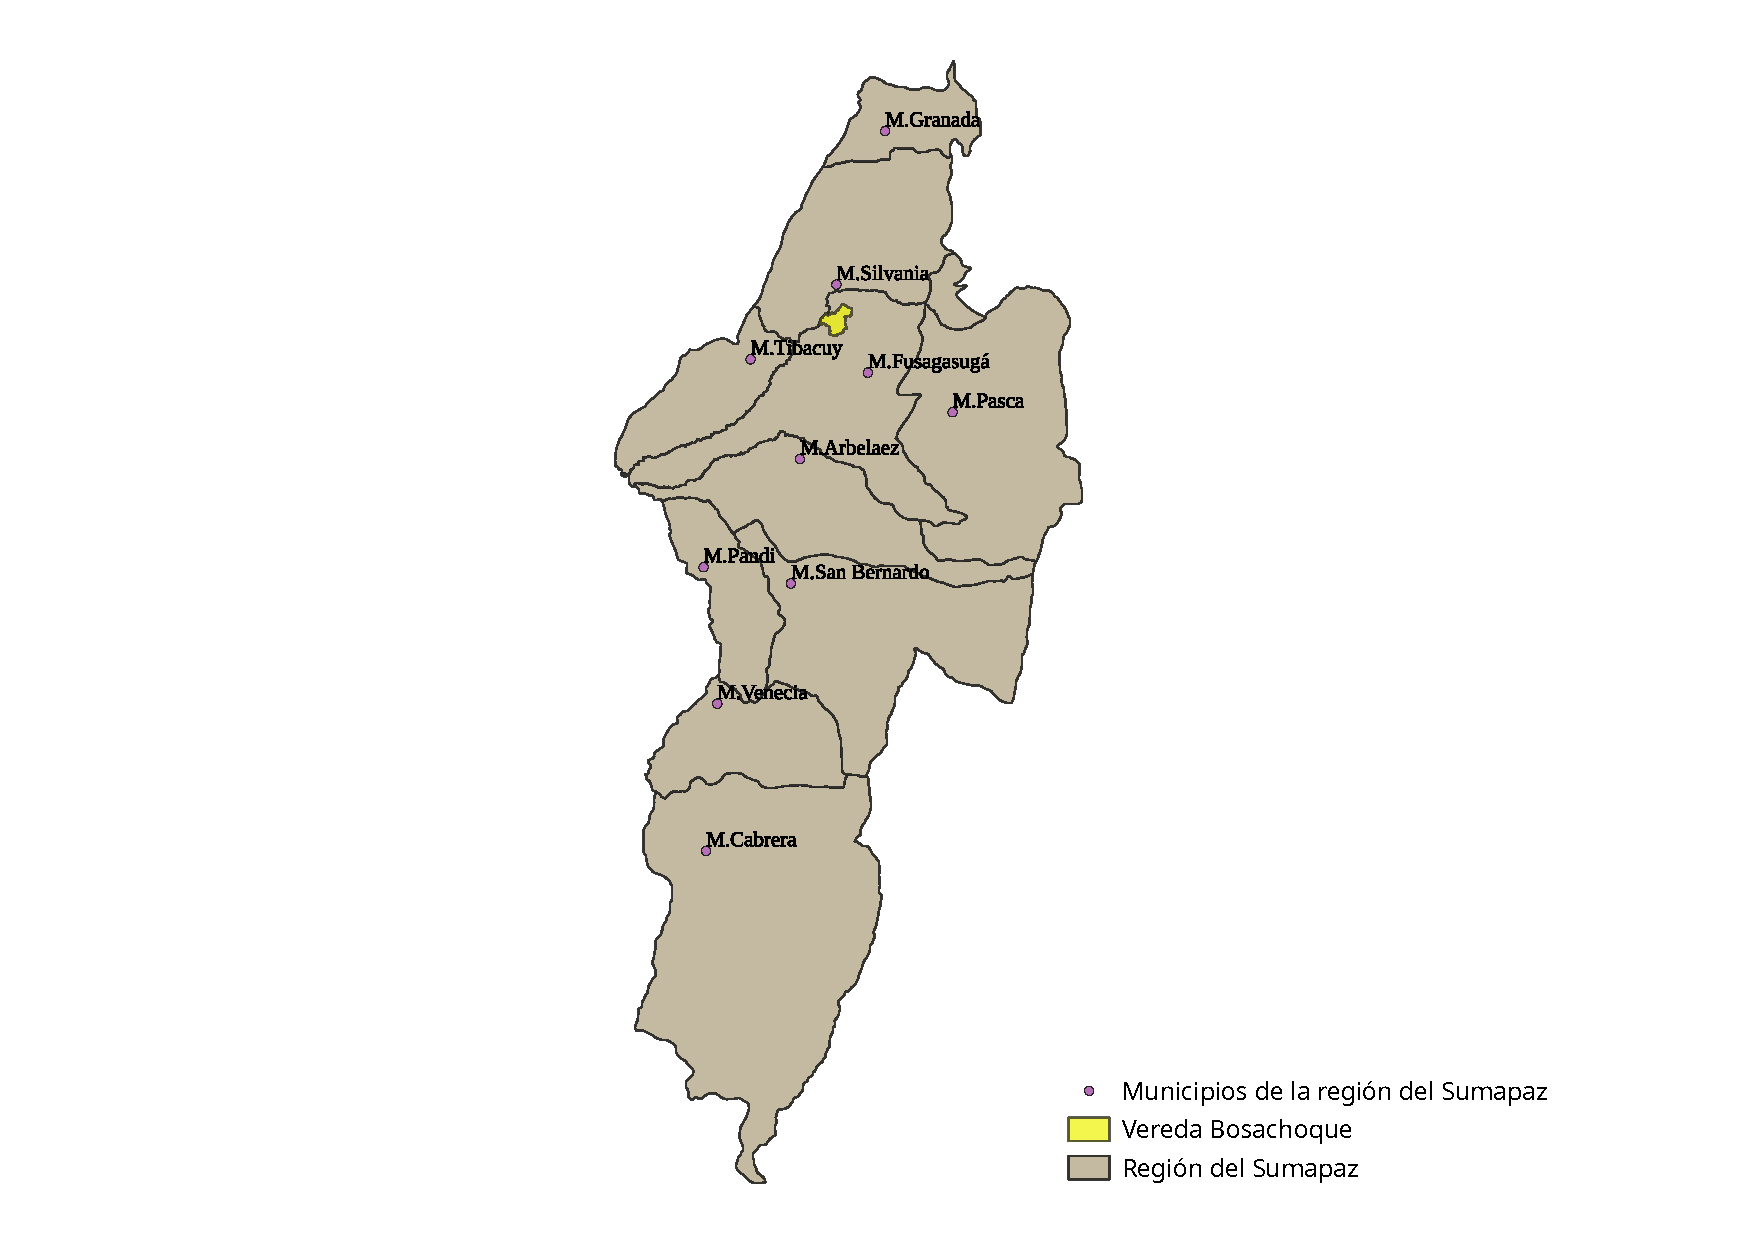
\includegraphics{Bosachoque_sumapaz.pdf}
\caption{Ubicación}
\end{figure}

En la Figura \ref{mylabel} se puede evidenciar con color amarillo la
vereda Bosachoque, lugar en el que se encuentra la red Libre de
Bosachoque y en color gris la región del Sumapaz, zona en dónde se desea
expandir la red.

\begin{itemize}
\tightlist
\item
  Solicitudes de cobertura:
\end{itemize}

Las solicitudes de cobertura se analizaron en las dos regiones, la red
actual y la futura expansión de la red.

Red Libre de Bosachoque:

De acuerdo con (Tobón) la red se implementó en la parte alta de la
vereda Bosachoque (Parte alta de la vía 40 express) instalando diez
puntos conectados a la torre de la vereda San José del Chocho en el
municipio de Silvania (Cundinamarca). Sin embargo, los habitantes de la
parte baja de la vereda no tenían acceso a la red, por lo tanto, las
personas solicitaron se les provea conectividad a Internet, acorde con
esto, se estableció en que coordenadas era posible instalar las antenas
y a partir de ahí verificar la población afectada.

\begin{figure}
\centering
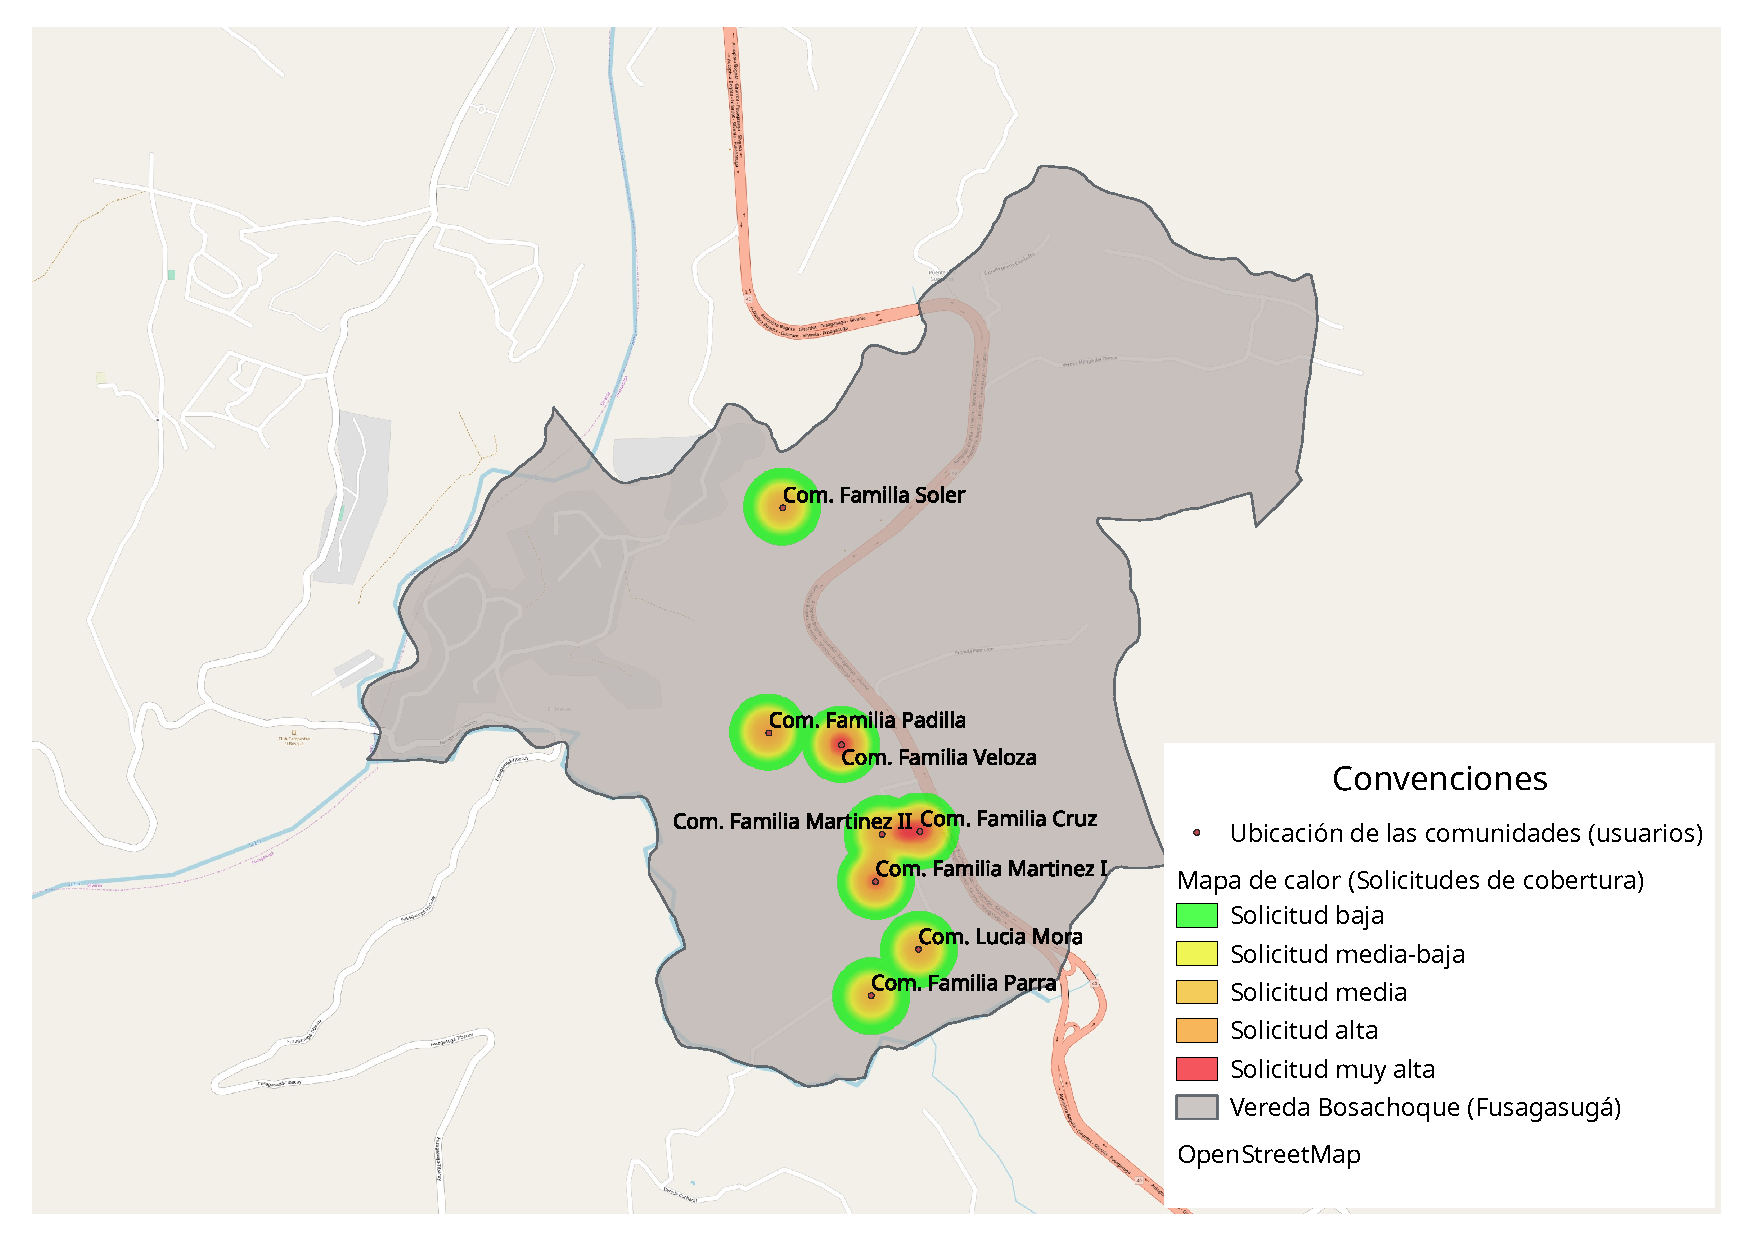
\includegraphics[width=1.00000\textwidth]{mc_b_solicitudes.pdf}
\caption{Mapa de calor, solicitud de cobertura Bosachoque
\label{mylabel}}
\end{figure}

En la figura \ref{mylabel} se puede encontrar el mapa de calor de las
solicitudes de cobertura en la vereda Bosachoque, entendiendo que el
color rojo es una solicitud más alta de cobertura y el color verde una
solicitud baja. Para realizar este mapa se tomó el dato de la
concentración de viviendas que podian acceder al servicio.

Región del Sumapaz:

Se desea expandir la red libre de Bosachoque a la región del Sumapaz,
para ello se plantea la interconexión de todas las Instituciones
Educativas Rurales de la región. A partir de este hecho, se obtienen las
coordenadas de cada Institución y la cantidad de estudiantes por cada
sede, (la información es proporcionada por la base de datos del
Ministerio de Educación Nacional), con estos datos se realiza el mapa de
calor.

\begin{figure}
\centering
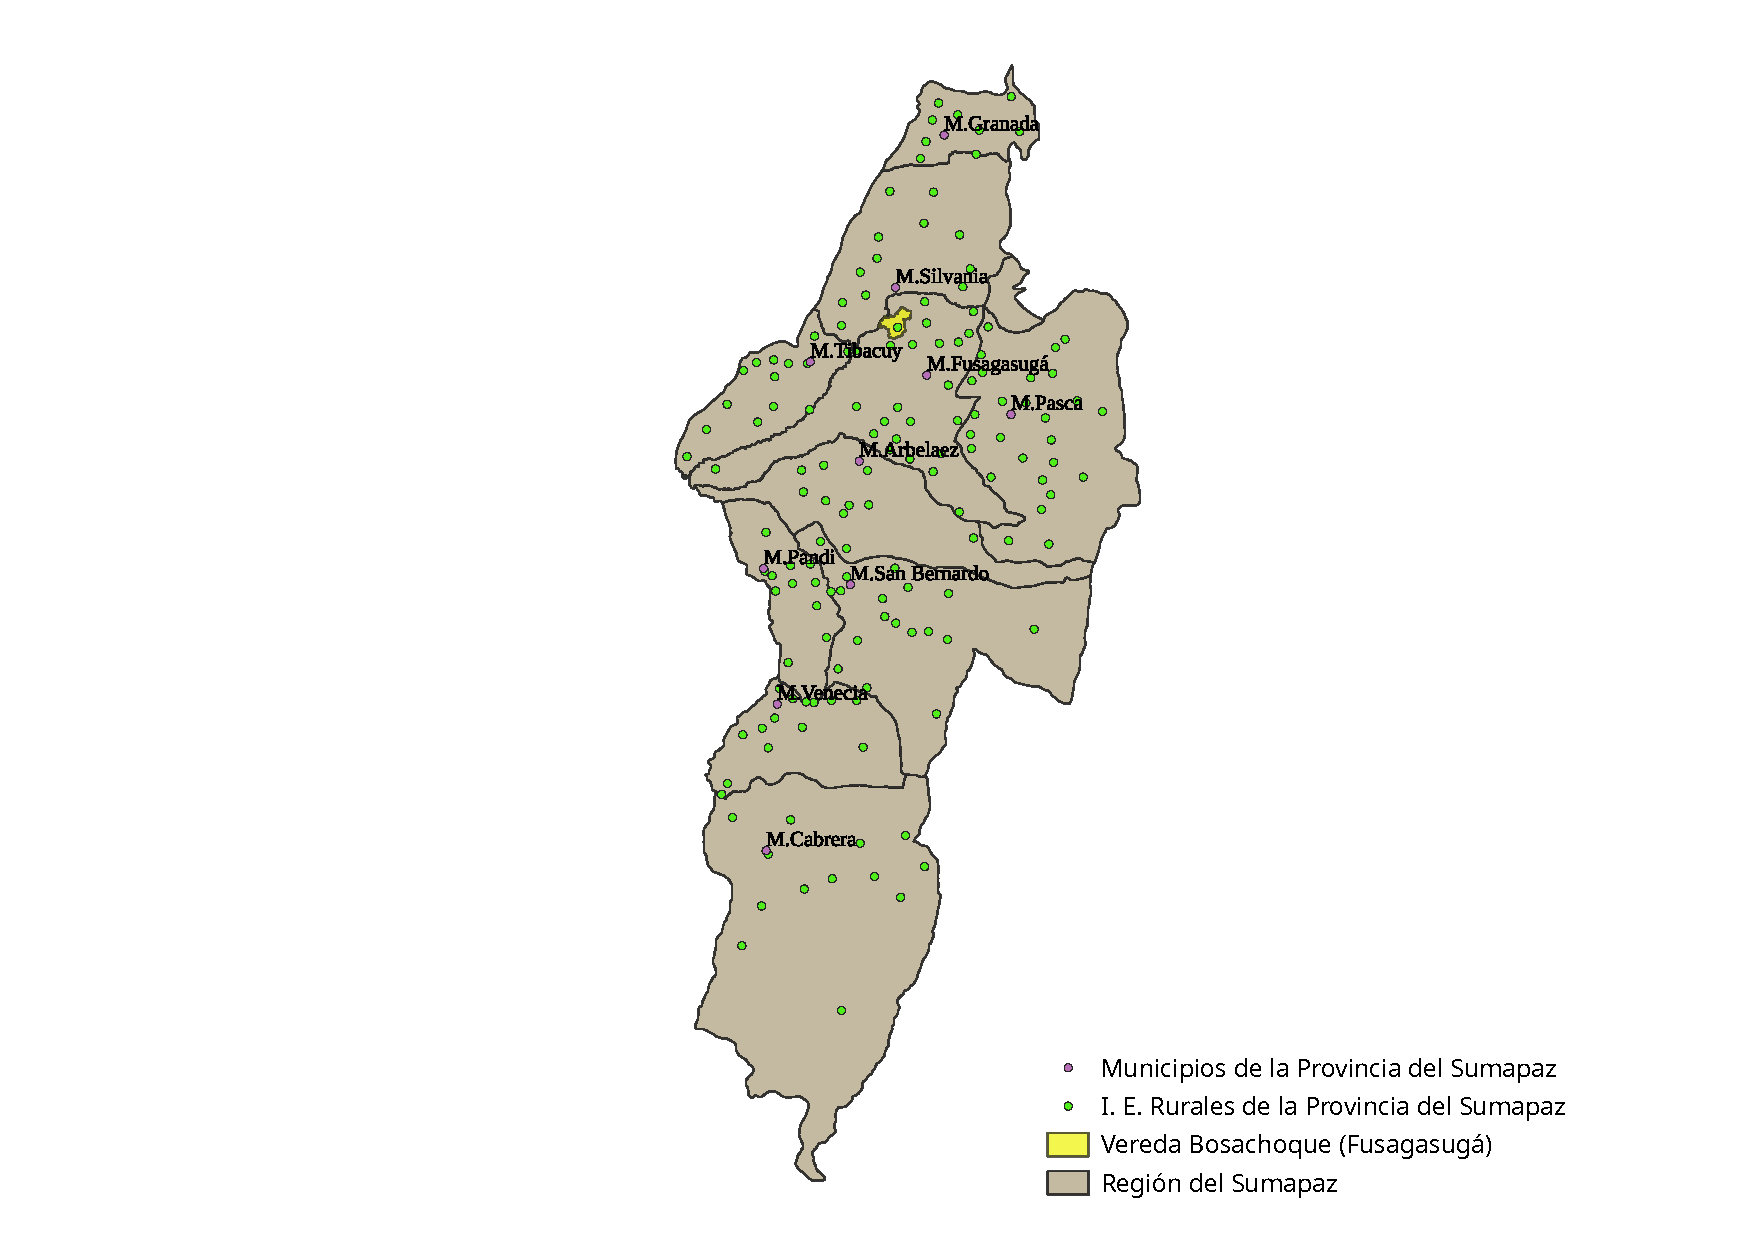
\includegraphics{Ubicacion_IE_Rurales.pdf}
\caption{Ubicación de las Instituciones Educativas Rurales en el
Sumapaz}
\end{figure}

En la figura n, se aprecia la ubicación de las escuelas rurales de la
región del Sumapaz (punto de color verde). Cabe resaltar que las I.E
Rurales están ubicadas en zonas apartadas o de dificil acceso, lo
anterior se aprecia mejor en la figura n.

\begin{figure}
\centering
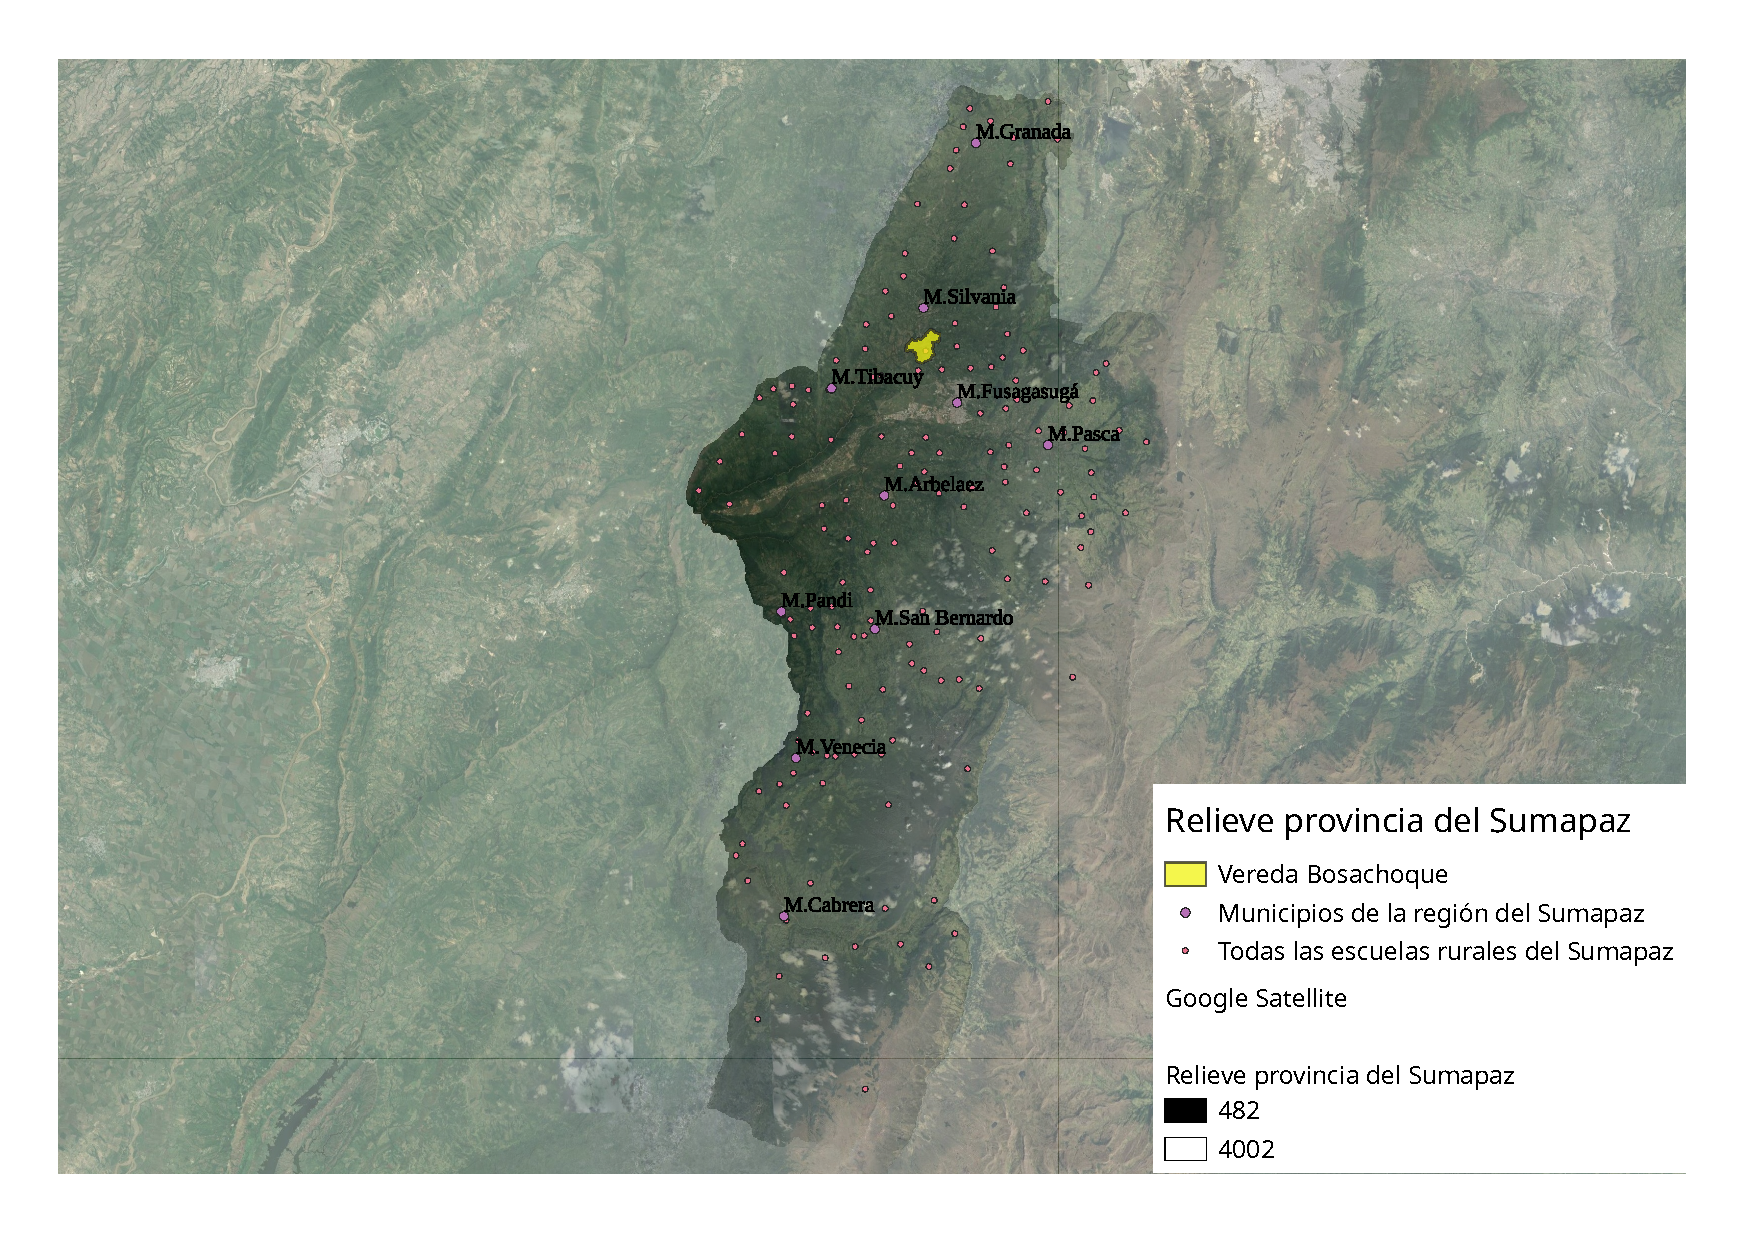
\includegraphics{relieve_sumapaz_escuela.pdf}
\caption{Relieve de la región del Sumapaz}
\end{figure}

\begin{figure}
\centering
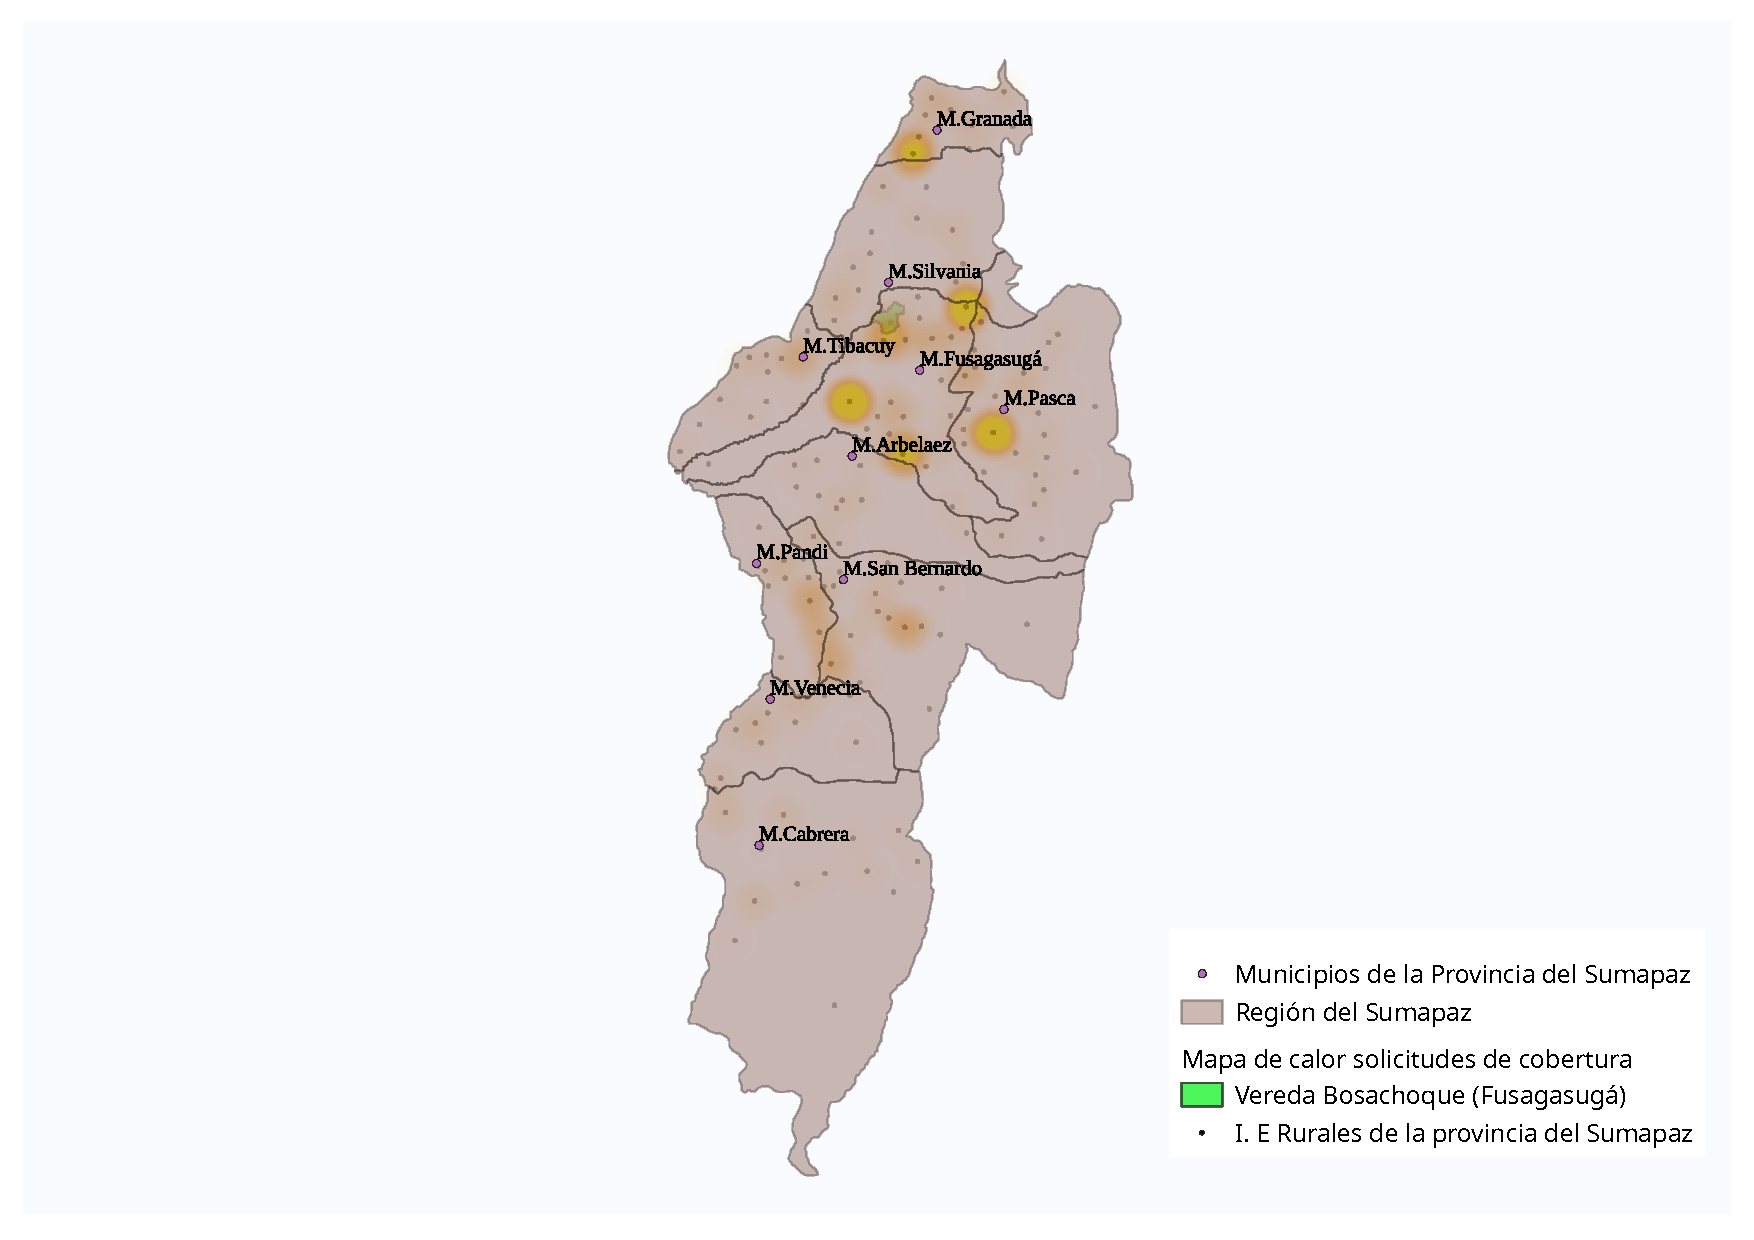
\includegraphics{calor_s.pdf}
\caption{Mapa de calor solicitudes en la región del Sumapaz}
\end{figure}

En la figura n, se puede visualizar el mapa de calor de las solicitudes
de servicio en la provincia del Sumapaz, entonces, a mayor cantidad de
estudiantes en la sede mayor será la cobertura, por ende, el color
amarillo simboliza una mayor concentración de estudiantes.

\begin{itemize}
\tightlist
\item
  Ubicación y desempeño de los usuarios actuales:
\end{itemize}

Partiendo que la red actual se encuentra ubicada en la vereda
Bosachoque, es allí dónde se genera el mapa de calor y así se determina
el desempeño que han tenido los nodos instalados.

\begin{figure}
\centering
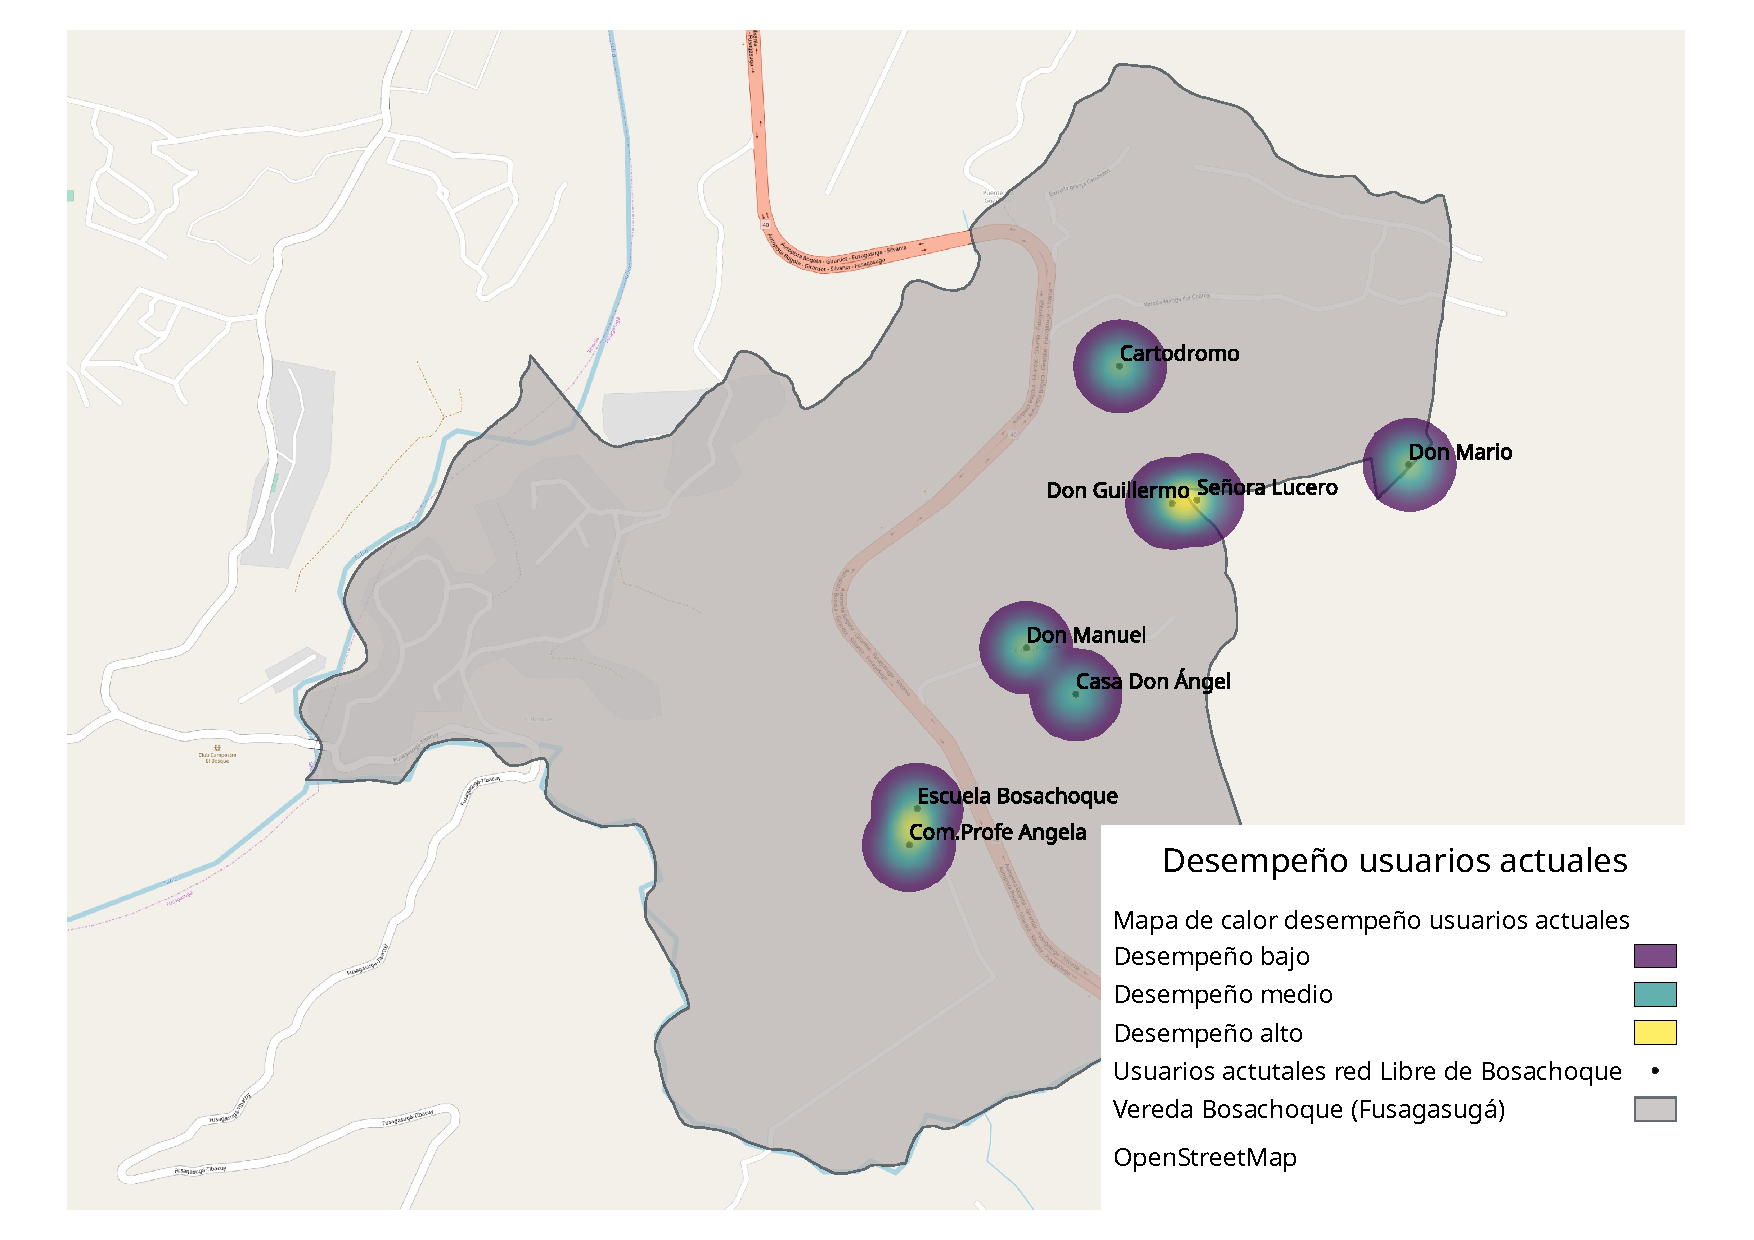
\includegraphics{Desempeno_usuarios_actuales_bosachoque.pdf}
\caption{Mapa de calor desempeño y ubicación de los usuarios actuales}
\end{figure}

De acuerdo con la figura n, el color amarillo indica los nodos con mejor
desempeño, el color azul brinda la perspectiva de un desempeño medio y
el color morado indica un desempeño bajo o sin desempeño. Por ende, la
antena ubicada en la ``Com. Profe Angela'' indica un desempeño alto, al
igual que ``Don Manuel'' y ``Don Mario'', sin embargo, los nodos
ubicados en ``Don Guillermo y Señora Lucero'' indican un desempeño alto,
esto dado la cercania de las dos antenas.

\section{Capitulo 4. Análisis de resultados y
discusión}\label{capitulo-4.-anuxe1lisis-de-resultados-y-discusiuxf3n}

\section{Conclusiones y trabajos
futuros}\label{conclusiones-y-trabajos-futuros}

\section{Bibliografía}\label{bibliografuxeda}

\end{document}
